\documentclass[11pt]{article}

\usepackage[letterpaper,margin=0.9in,headheight=22pt,headsep=0.23in,footskip=0.38in]{geometry}
\usepackage[T1]{fontenc}
\usepackage{newtxtext,newtxmath}
\usepackage{microtype}
\usepackage{booktabs}
\usepackage{longtable}
\usepackage{tabularx}
\usepackage{array}
\usepackage{ragged2e}
\usepackage{makecell}
\usepackage{graphicx}
\usepackage{amsmath}
\usepackage{siunitx}
\usepackage[table]{xcolor}
\usepackage{caption}
\usepackage{fancyhdr}
\usepackage{lastpage}
\usepackage{titlesec}
\usepackage{xurl}
\usepackage{hyperref}

\definecolor{HydroNavy}{HTML}{0B2E59}
\definecolor{HydroBlue}{HTML}{005EA8}
\definecolor{HydroPale}{HTML}{EAF2F8}
\definecolor{HydroGray}{HTML}{5E6A71}

\hypersetup{
  colorlinks=true,
  linkcolor=HydroBlue,
  citecolor=HydroBlue,
  urlcolor=HydroBlue,
  pdfborder={0 0 0},
  pdftitle={HydroPol2D Validation Report},
  pdfauthor={Marcus N\'obrega},
  pdfsubject={Validation of HydroPol2D computational modules},
  pdfkeywords={HydroPol2D, validation, hydrology, hydrodynamics}
}

\titleformat{\section}
  {\Large\bfseries\color{HydroNavy}}
  {\thesection}{0.8em}{}
\titleformat{\subsection}
  {\large\bfseries\color{HydroNavy}}
  {\thesubsection}{0.7em}{}
\titlespacing*{\section}{0pt}{1.7ex plus .3ex minus .2ex}{0.8ex}
\titlespacing*{\subsection}{0pt}{1.35ex plus .2ex minus .2ex}{0.55ex}

\pagestyle{fancy}
\fancyhf{}
\fancyhead[L]{\small\color{HydroGray}HydroPol2D}
\fancyhead[R]{\small\color{HydroGray}Validation Report}
\fancyfoot[C]{\small\color{HydroGray}\thepage\ of \pageref{LastPage}}
\renewcommand{\headrulewidth}{0.35pt}
\renewcommand{\headrule}{\hbox to\headwidth{\color{HydroBlue}\leaders\hrule height \headrulewidth\hfill}}

\captionsetup{
  font=small,
  labelfont={bf,color=HydroNavy},
  labelsep=period,
  skip=6pt,
  justification=raggedright,
  singlelinecheck=false
}
\setlength{\LTpre}{0.65\baselineskip}
\setlength{\LTpost}{0.65\baselineskip}
\renewcommand{\arraystretch}{1.14}
\setlength{\tabcolsep}{5pt}
\newcolumntype{L}[1]{>{\RaggedRight\arraybackslash}p{#1}}
\newcolumntype{C}[1]{>{\Centering\arraybackslash}p{#1}}
\newcolumntype{R}[1]{>{\RaggedLeft\arraybackslash}p{#1}}
\newcolumntype{Y}{>{\RaggedRight\arraybackslash}X}
\newcommand{\thcell}[1]{\makecell[c]{\bfseries #1}}
\newcommand{\pass}{\textcolor{green!45!black}{pass}}
\newcommand{\notapplicable}{\textcolor{HydroGray}{not applicable}}
\newcommand{\filepath}[1]{{\small\ttfamily\Urlmuskip=0mu plus 1mu\relax\path{#1}}}
\emergencystretch=3em

\newcommand{\pending}{\textcolor{orange}{Pending current-code rerun}}
\newcommand{\diagnostic}{\textcolor{red}{Diagnostic only}}
\newcommand{\ready}{\textcolor{green!50!black}{Report-ready}}

\begin{document}
\hypersetup{pageanchor=false}
\begin{titlepage}
\thispagestyle{empty}
\centering
\vspace*{1.55in}
{\color{HydroBlue}\rule{0.18\textwidth}{1.4pt}}\par
\vspace{0.36in}
{\fontsize{30}{35}\selectfont\bfseries\color{HydroNavy} HydroPol2D}\par
\vspace{0.12in}
{\fontsize{19}{24}\selectfont\color{HydroGray} Validation Report}\par
\vspace{0.34in}
{\color{HydroBlue}\rule{0.56\textwidth}{0.7pt}}\par
\vfill
{\large\bfseries Marcus N\'obrega, Ph.D.}\par
\vspace{0.08in}
{\normalsize HydroPol2D developer}\par
\vspace{0.24in}
\small
\href{https://github.com/marcusnobrega-eng/HydroPol2D}{GitHub}
\enspace|\enspace
\href{https://www.linkedin.com/in/marcus-n%C3%B3brega-744b61138/}{LinkedIn}
\enspace|\enspace
\href{https://scholar.google.com/scholar?q=Marcus+N%C3%B3brega}{Google Scholar}
\enspace|\enspace
\href{https://www.researchgate.net/profile/Marcus-Gomes-Jr}{ResearchGate}
\enspace|\enspace
\href{https://orcid.org/0000-0002-8250-8195}{ORCID}\par
\vfill
{\small\color{HydroGray}\today}
\end{titlepage}
\setcounter{page}{1}
\hypersetup{pageanchor=true}

\begin{abstract}
This report documents the HydroPol2D validation suite. It evaluates formulas and numerical dynamics using analytical solutions, independent reference calculations, exact bookkeeping tests, benchmark hydrographs, and synthetic parameter-recovery cases. The shared spatial case-study domain is a V-tilted synthetic catchment, used to embed module-scale tests in a consistent HydroPol2D grid. The report includes canopy interception, snow, infiltration, evapotranspiration, groundwater and recharge, hydrodynamics, routing alternatives, Neal (2012) channel-subgrid hydraulics, reservoirs, boundary conditions, spatial rainfall, water-quality buildup and washoff, and human risk. Model results are compared with analytical solutions, independent calculations, exact storage ledgers, or documented fine-grid numerical references.
\end{abstract}

\section{Report Status}
This report evaluates HydroPol2D equations, storage updates, boundary bookkeeping, and numerical behavior against known or independently computed reference behavior. Numerical results are included only when current-code outputs have been generated and compared with a documented reference.

\section{Validation Scope}
\label{sec:validation-scope}
The validation suite evaluates formulas and dynamics using analytical solutions, independent reference calculations, manufactured or simplified benchmark solutions, exact bookkeeping, and synthetic inverse-modeling cases. These tests establish computational verification and benchmark validation of individual modules. Synthetic inverse modeling is used for parameter recovery: known synthetic observations are generated from known parameters, and HydroPol2D or its diagnostic routines must recover those parameters within documented tolerances.

The execution registry is maintained in \filepath{Validation/Validation_Cases.csv}. Analytical and bookkeeping reference outputs are stored under \filepath{Validation/Reference_Outputs/Validation}.

The shared spatial case-study domain is the V-tilted synthetic catchment under \filepath{Validation/VTilted_Catchment}. The analytical or independent reference solution remains the truth source; the V-tilted catchment provides a consistent DEM, LAI, soil, land-cover, groundwater, channel, and boundary-condition context for HydroPol2D runs. Ritter dam-break and non-breaking-wave benchmarks retain their own geometries because their analytical comparisons require specialized domains.

\section{Case-study Overview}
\label{sec:case-study}
The shared case-study domain is a synthetic V-tilted catchment. It has a central channel strip and two lateral hillslopes that drain toward the channel, with a longitudinal slope toward the outlet. The domain provides spatial heterogeneity without introducing field-data uncertainty.

The generated raster grid has 50 rows by 81 columns at \SI{20}{\meter} resolution. Three zones are used in the first canopy test: a left hillslope with sparse vegetation, a channel strip with no canopy, and a right hillslope with denser vegetation. Table~\ref{tab:vtilted-domain} summarizes the domain zones used in the completed canopy case.

\begin{table}[htbp]
\centering
\caption{V-tilted catchment zones used in the canopy interception test.}
\label{tab:vtilted-domain}
\begin{tabular}{lrrr}
\toprule
Zone & Cells & LAI & Initial soil moisture (mm) \\
\midrule
Left hillslope & 2000 & 0.5 & 50 \\
Channel strip & 100 & 0.0 & 30 \\
Right hillslope & 1950 & 2.0 & 70 \\
\bottomrule
\end{tabular}
\end{table}

\section{Validation Methods}
\label{sec:methods}
Each validation case must define: model flags, input data, expected behavior, diagnostic outputs, metrics, acceptance thresholds, and report figure/table identifiers. The standard diagnostic bundle is:
\begin{itemize}
  \item mass-balance table;
  \item time-series and profile comparisons where applicable;
  \item raster maps or one-dimensional profiles for spatial behavior;
  \item metric summary table;
  \item pass/fail table with threshold references.
\end{itemize}

Storage and algebraic unit tests use exact mass closure as the primary criterion. The default tolerance is \SI{1e-6}{\cubic\meter} for unit tests or \SI{0.01}{\percent} of input volume when the volume scale makes an absolute tolerance inappropriate. Full-domain cases target final water-balance error below \SI{0.1}{\percent}. Hydrograph and profile benchmarks report root-mean-square error, mean absolute error, maximum error, relative $L_2$ error, peak timing error, peak magnitude error, and Nash-Sutcliffe efficiency where applicable.

No case is report-ready when the diagnostic summary contains unexplained \texttt{NaN} values, undocumented residuals, or missing pass/fail criteria.

\subsection{Evidence Hierarchy}
\label{sec:validation-evidence}
The preferred evidence hierarchy is:
\begin{enumerate}
  \item analytical or semi-analytical solution;
  \item independently computed reference formula;
  \item manufactured or simplified benchmark solution;
  \item synthetic inverse-modeling parameter recovery;
  \item cross-model comparison against a simple trusted solver.
\end{enumerate}
The first three are the main evidence sources. Synthetic inverse modeling is useful for checking identifiability and parameter sensitivity, but it must not be presented as field validation.

\subsection{Reference Cases}
\label{sec:validation-reference-cases}
The suite includes explicit analytical and reference cases for the main computational modules. Priority cases include Green-Ampt and Philip infiltration, FAO-style ET with availability limits, configurable snow storage and melt, canopy bucket storage, linear-reservoir groundwater recession, Ritter and non-breaking-wave hydrodynamics, corrected kinematic/diffusive routing, Manning/channel conveyance, reservoir rating-curve depletion, exact inflow/stage volume bookkeeping, tiny raster rainfall totals, analytical wash-off, and deterministic human-risk thresholds.

For HydroPol2D runs, these cases should be embedded in the v-tilted synthetic catchment wherever possible. The report must still compare model outputs against the analytical/reference solution, not against the v-tilted domain itself.

\section{Validation Matrix}
\label{sec:matrix}
The registry is maintained in \filepath{Validation/Validation_Cases.csv}. Table~\ref{tab:validation-matrix} summarizes the current evidence chain.

\small
\renewcommand{\arraystretch}{1.16}
\setlength{\tabcolsep}{4pt}
\begin{longtable}{@{}L{0.185\linewidth}L{0.305\linewidth}L{0.315\linewidth}C{0.14\linewidth}@{}}
\caption{HydroPol2D validation matrix.}
\label{tab:validation-matrix}\\
\toprule
\rowcolor{HydroPale}
\thcell{Component} & \thcell{Reference evidence} & \thcell{Case-study domain} & \thcell{Status} \\
\midrule
\endfirsthead
\toprule
\rowcolor{HydroPale}
\thcell{Component} & \thcell{Reference evidence} & \thcell{Case-study domain} & \thcell{Status} \\
\midrule
\endhead
Canopy interception & Independent canopy-bucket reference & V-tilted zones & \ready \\
Snow & Independent snow formula/storage reference & V-tilted zones & \ready \\
Infiltration & Independent layered storage and Darcy--van Genuchten regime references & V-tilted hillslope cells & \ready \\
Evapotranspiration & Independent reference ET and extraction limits & V-tilted zones & \ready \\
Groundwater/recharge & Analytical recharge/capillary references, Dupuit hillslope, linearized Boussinesq hillslope, and fine-timestep Boussinesq reference & V-tilted and idealized hillslope profiles & \ready \\
Hydrodynamics & Full-momentum analytical benchmarks; local-inertial, CA, kinematic, and diffusive diagnostics & V-tilted and specialized benchmark domains & \ready \\
Routing alternatives & Corrected kinematic/diffusive solvers pass plane, V-tilted, and stage checks; Ritter remains diagnostic & V-tilted slopes & \ready \\
Neal (2012) channel-subgrid hydraulics & Fine-grid local-inertial references for in-bank, composite-channel, and staged-overbank dynamics & Synthetic straight and compound-channel reaches & \ready \\
Reservoir/control structures & Rating-curve storage ODE & Idealized reservoir/control cell & \ready \\
Inflow hydrograph BC & Exact imposed-volume bookkeeping & Rectangular full-momentum domain & \ready \\
Stage hydrograph BC & Prescribed-stage enforcement and volume bookkeeping & Rectangular full-momentum domain & \ready \\
Spatial rainfall & Exact raster rainfall totals & Tiny GeoTIFF raster stack & \ready \\
Water quality & Analytical SWMM-style build-up/wash-off ODE & Single- and two-cell module drivers & \ready \\
Human risk & Independent drag/friction and force-balance references & Synthetic depth/velocity grids & \ready \\
\bottomrule
\end{longtable}
\normalsize

\section{Canopy Interception}
\label{sec:canopy}
The canopy interception case isolates the HydroPol2D canopy storage routine before coupled infiltration, runoff, or groundwater processes are considered. The test uses the v-tilted catchment zones described in Table~\ref{tab:vtilted-domain}. The left hillslope has LAI = 0.5, the channel strip has LAI = 0, and the right hillslope has LAI = 2.0. A representative \SI{20}{\meter} by \SI{20}{\meter} cell is used for volume conversion.

\subsection{Canopy Method}
\label{sec:canopy-method}
The canopy case driver calls the HydroPol2D interception routine directly. The independent reference follows the same intended canopy-bucket bookkeeping. For each zone and time step, maximum canopy storage is
\begin{equation}
S_{\max} = C \, LAI,
\end{equation}
where $C=\SI{0.2}{\milli\meter}$ per LAI unit. Potential canopy evaporation is reduced by the previous fractional canopy storage:
\begin{equation}
E_t = \min\left(\frac{S_{t-1}}{S_{\max}} E_{p,t},\, P_t + S_{t-1}\right),
\end{equation}
with $E_t=0$ when $S_{\max}=0$. Temporary storage before throughfall is
\begin{equation}
S^*_t = S_{t-1} + P_t - E_t.
\end{equation}
Throughfall and final canopy storage are then
\begin{equation}
T_t = \max(S^*_t - S_{\max},0), \qquad S_t = \min(S^*_t,S_{\max}).
\end{equation}
Stemflow is not active in the current HydroPol2D routine for this test. The diagnostic residual is
\begin{equation}
r_t = (S_t-S_{t-1}) - (P_t - E_t - T_t).
\end{equation}

The forcing sequence includes canopy filling, throughfall after capacity is exceeded, evaporation drawdown, and an LAI=0 bypass condition in the channel strip. The reference output is stored in \filepath{Validation/Reference_Outputs/Validation/canopy_bucket/VAL-CANOPY-001_reference.csv}; the MATLAB HydroPol2D output is stored in \filepath{Validation/Canopy_Interception/SingleCell_Storage_Balance/Outputs/Validation/HydroPol2D_Canopy_Model.csv}.

\subsection{Canopy Results}
\label{sec:canopy-results}
The HydroPol2D MATLAB canopy output matched the independent reference to round-off precision. Table~\ref{tab:canopy-results} summarizes the diagnostic metrics. The case is marked report-ready because the benchmark comparison, mass-balance check, and NaN check all passed.

\begin{table}[htbp]
\centering
\caption{Canopy interception validation metrics for case VAL-CANOPY-001.}
\label{tab:canopy-results}
\begin{tabular}{lrrl}
\toprule
Metric & Value & Threshold & Pass \\
\midrule
Canopy storage RMSE (mm) & $1.50\times10^{-17}$ & $1.0\times10^{-9}$ & yes \\
Throughfall RMSE (mm) & $1.31\times10^{-17}$ & $1.0\times10^{-9}$ & yes \\
Evaporation RMSE (mm) & $7.31\times10^{-18}$ & $1.0\times10^{-9}$ & yes \\
Maximum storage error (mm) & $5.55\times10^{-17}$ & $1.0\times10^{-9}$ & yes \\
Maximum throughfall error (mm) & $5.55\times10^{-17}$ & $1.0\times10^{-9}$ & yes \\
Maximum evaporation error (mm) & $2.78\times10^{-17}$ & $1.0\times10^{-9}$ & yes \\
Maximum mass residual (\si{\cubic\meter}) & $2.22\times10^{-17}$ & $1.0\times10^{-6}$ & yes \\
\bottomrule
\end{tabular}
\end{table}

The pass/fail summary reports \texttt{status = pass}, \texttt{mass\_balance\_pass = true}, \texttt{benchmark\_pass = true}, \texttt{nan\_check\_pass = true}, and \texttt{report\_ready = true}. This validates the canopy interception formula and storage bookkeeping for the tested v-tilted-zone conditions. It does not validate field canopy interception behavior, because no field throughfall or stemflow observations are used in validation.

\section{Snow Module}
\label{sec:snow}
The snow validation applies prescribed cold, transitional, and warm forcings to representative v-tilted zones. The case calls \texttt{Snow\_Model\_Function.m} directly and compares the MATLAB output against an independent Python reference that mirrors the active HydroPol2D formulas. The test checks rain/snow partitioning, snow water equivalent (SWE), snow depth, snow density, melt, sublimation, and snowpack mass closure.

\subsection{Snow Method}
\label{sec:snow-method}
The active precipitation partition in \texttt{Snow\_Model\_Function.m} uses a linear snow fraction between \SI{4}{\celsius} and \SI{7}{\celsius}:
\begin{equation}
f_s = \min\left(\max\left(\frac{7 - T_a}{7-4},0\right),1\right), \qquad
P_s = f_s P, \qquad P_r = P - P_s .
\end{equation}
This is an implementation detail: the routine accepts a threshold argument, but the active partition currently uses the hard-coded 4--7~\si{\celsius} transition. validation therefore validates the implemented formula, not a configurable threshold formulation.

After snowfall is added to SWE, the routine computes net radiation, updates density and diagnostic snow depth from previous SWE, and computes melt as the sum of degree-day and radiation terms bounded by available SWE:
\begin{equation}
M_t = \min\left(SWE_{t-1}+P_s,\,
\max\left(DDF\,T_a + \frac{(1-\alpha)Q_{net}}{334},0\right)\right).
\end{equation}
Sublimation is computed from wind speed and a vapor-pressure-gradient term and is also bounded by available SWE after melt. The storage update is
\begin{equation}
SWE_t = SWE_{t-1} + P_s - M_t - E_s,
\end{equation}
with diagnostic residual
\begin{equation}
r_t = SWE_{t-1} + P_s - M_t - E_s - SWE_t.
\end{equation}

The reference forcing uses three v-tilted scenarios: left hillslope, channel strip, and right hillslope. The temperatures span fully snow-dominated, transitional mixed rain/snow, and rain-only conditions. The reference output is stored in \filepath{Validation/Reference_Outputs/Validation/snow_degree_day/VAL-SNOW-001_reference.csv}; the MATLAB output is stored in \filepath{Validation/Snow/ColdWarmPartition_Melt/Outputs/Validation/HydroPol2D_Snow_Model.csv}.

\subsection{Snow Results}
\label{sec:snow-results}
The HydroPol2D MATLAB snow output matched the independent reference to round-off precision. Table~\ref{tab:snow-results} summarizes the diagnostic metrics. The case is marked report-ready because the benchmark comparison, mass-balance check, and NaN check all passed.

\begin{table}[htbp]
\centering
\caption{Snow-module validation metrics for case VAL-SNOW-001.}
\label{tab:snow-results}
\begin{tabular}{lrrl}
\toprule
Metric & Value & Threshold & Pass \\
\midrule
SWE RMSE (mm) & $1.59\times10^{-14}$ & $1.0\times10^{-8}$ & yes \\
Melt RMSE (mm) & $1.27\times10^{-14}$ & $1.0\times10^{-8}$ & yes \\
Snowfall RMSE (mm) & $7.54\times10^{-15}$ & $1.0\times10^{-8}$ & yes \\
Rainfall RMSE (mm) & $4.19\times10^{-16}$ & $1.0\times10^{-8}$ & yes \\
Sublimation RMSE (mm) & $1.86\times10^{-20}$ & $1.0\times10^{-8}$ & yes \\
Snow density RMSE (\si{\kilogram\per\cubic\meter}) & $1.78\times10^{-13}$ & $1.0\times10^{-8}$ & yes \\
Maximum mass residual (\si{\cubic\meter}) & $0.0$ & $1.0\times10^{-6}$ & yes \\
\bottomrule
\end{tabular}
\end{table}

The pass/fail summary reports \texttt{status = pass}, \texttt{mass\_balance\_pass = true}, \texttt{benchmark\_pass = true}, \texttt{nan\_check\_pass = true}, and \texttt{report\_ready = true}. This validates the implemented snow partition, melt, sublimation, density, depth, and SWE bookkeeping formulas for the tested v-tilted-zone conditions. It does not validate field snowpack behavior because no snow-pillow, snow-course, or remotely sensed SWE observations are used in validation.

\section{Infiltration}
\label{sec:infiltration}
The infiltration validation uses the v-tilted catchment as the shared validation spatial context, but the truth source is an independent MATLAB reference driver that evaluates the intended infiltration and layered-storage bookkeeping outside the full hydrodynamic solver. This is deliberate: validation asks whether the equations and storage dynamics behave correctly before interpreting routed hydrographs or field-scale calibration.

\subsection{Infiltration Method}
\label{sec:infiltration-method}
Seven regimes were tested with the current code using \texttt{run\_vtilted\_infiltration\_validation\_suite.m}. The test grid and land-cover/soil zones come from \texttt{Validation\_VTilted\_Catchment}; the infiltration cases are listed in \texttt{Infiltration\_Case\_Registry.csv}. The suite evaluates: no-infiltration bypass, supply-limited rainfall, capacity-limited intake, finite-storage saturation excess, delayed layered percolation and recharge, shallow-groundwater saturation excess, and spatial soil contrast. The hydraulic parameters were reset to physically interpretable USDA-style sandy-loam, loam, and clay-loam values using the Mualem--van Genuchten framework \cite{Mualem1976,VanGenuchten1980,CarselParrish1988}. Layer multipliers are used only to represent plausible structured topsoil, compacted soil, or moderately slower subsoil conductivity.

For each time step, precipitation is partitioned into infiltration, surface excess, layer storage, and recharge. The independent reference enforces the same intended top-down layer order used by the implemented model: near-surface layer, root-zone layer, transmission layer, and groundwater recharge when the vadose storage is full and recharge is enabled. The diagnostic closure residual is
\begin{equation}
r_t = P_t - F_t - R_t - G_t - \Delta S_t,
\end{equation}
where $P_t$ is precipitation, $F_t$ is infiltrated water retained in the vadose layers, $R_t$ is surface excess/runoff supply, $G_t$ is recharge, and $\Delta S_t$ is the change in vadose storage. The primary acceptance checks are physically distinct rather than one aggregate score: supply-limited cases must infiltrate all rainfall, capacity-limited cases must generate excess when rainfall exceeds intake, storage-limited cases must saturate the vadose store, recharge cases must show delayed transmission and recharge, and spatial-contrast cases must generate more excess from the low-conductivity zone.

A coupled HydroPol2D full-domain runoff-control case was also executed with adaptive hydrodynamic stepping. It completed stably after allowing the inertial solver to reduce the internal time step from the registry forcing interval. That coupled run is retained as diagnostic only because the full routed water-balance benchmark has not yet been defined for this infiltration section.

\subsection{Infiltration Results}
\label{sec:infiltration-results}
All seven independent infiltration-regime cases passed after the soil properties were replaced with physically consistent texture-based parameters. Table~\ref{tab:infiltration-results} summarizes the main diagnostics. Closure errors were zero or round-off scale, with the largest residual equal to $1.23\times10^{-11}$~mm in the layered percolation case. The pass/fail file reports \texttt{status = pass} and \texttt{report\_ready = true} for every independent-regime case.

\begin{table}[htbp]
\centering
\caption{Infiltration validation diagnostics for the v-tilted validation cases.}
\label{tab:infiltration-results}
\small
\begin{tabular}{llrrrrr}
\toprule
Case & Regime & Rain & Infil. & Runoff & Recharge & Closure \\
 & & (mm) & (mm) & (mm) & (mm) & (mm) \\
\midrule
VAL-INFIL-VT-000 & No infiltration & 60.0 & 0.0 & 60.0 & 0.0 & 0.0 \\
VAL-INFIL-VT-001 & Supply limited & 10.0 & 10.0 & 0.0 & 0.0 & 0.0 \\
VAL-INFIL-VT-002 & Capacity limited & 120.0 & 34.157 & 85.843 & 0.0 & $1.71\times10^{-13}$ \\
VAL-INFIL-VT-003 & Storage limited & 180.0 & 72.5 & 107.5 & 0.0 & 0.0 \\
VAL-INFIL-VT-004 & Layered percolation & 384.0 & 384.0 & 0.0 & 197.614 & $1.23\times10^{-11}$ \\
VAL-INFIL-VT-005 & Shallow groundwater & 150.0 & 75.0 & 75.0 & 22.683 & $-2.84\times10^{-14}$ \\
VAL-INFIL-VT-006 & Spatial soil contrast & 120.0 & 77.880 & 42.120 & 0.0 & $7.11\times10^{-15}$ \\
\bottomrule
\end{tabular}
\end{table}

\begin{figure}[htbp]
\centering
\includegraphics[width=\linewidth]{../../HydroPol2D/Validation/Infiltration/VTilted_Infiltration/Outputs/Validation/Figures/VTilted_Infiltration_Hydrograph_Overview.pdf}
\caption{V-tilted infiltration hydrograph overview. Rates are shown in \si{\milli\meter\per\hour}; black lines are rainfall, blue lines are runoff or surface-excess generation, and green lines are recharge. The spatial-contrast case also shows the high-conductivity response with a dashed blue line.}
\label{fig:infiltration-hydrographs}
\end{figure}

\begin{figure}[htbp]
\centering
\includegraphics[width=\linewidth]{../../HydroPol2D/Validation/Infiltration/VTilted_Infiltration/Outputs/Validation/Figures/VTilted_Infiltration_Rate_Overview.pdf}
\caption{V-tilted infiltration-rate overview. Rates are shown in \si{\milli\meter\per\hour}; black lines are rainfall and red lines are accepted infiltration. The spatial-contrast case also shows the high-conductivity accepted-infiltration response with a dashed red line.}
\label{fig:infiltration-rates}
\end{figure}

The results show the expected behavior under recognizable soil textures. In the supply-limited sandy-loam case, the full \SI{10}{\milli\meter} rainfall input infiltrated. In the capacity-limited clay-loam case, only \SI{34.157}{\milli\meter} infiltrated and \SI{85.843}{\milli\meter} became excess, consistent with rainfall exceeding hydraulic intake capacity. In the shallow sandy-loam storage case, the vadose store filled to \SI{86.25}{\milli\meter} and subsequent rainfall became saturation-excess runoff. In the moist sandy-loam percolation case, all \SI{384}{\milli\meter} of rainfall infiltrated; \SI{197.614}{\milli\meter} drained to recharge and \SI{301.386}{\milli\meter} remained in vadose storage, producing a gradual recharge rise rather than an immediate pulse. In the shallow-groundwater loam case, limited vadose capacity produced \SI{75}{\milli\meter} of excess and \SI{22.683}{\milli\meter} of recharge. The spatial-contrast case produced more excess from the compacted low-conductivity sandy-loam realization than from the high-conductivity realization.

Figures~\ref{fig:infiltration-hydrographs} and~\ref{fig:infiltration-rates} show the rate diagnostics used to visually inspect the same cases. Individual per-case plots with hydrograph, infiltration-rate, capacity, and layer-storage panels are stored in \filepath{Validation/Infiltration/VTilted_Infiltration/Outputs/Validation/Figures}. This validates the implemented infiltration bookkeeping and layered-soil dynamics for the tested validation regimes. It does not validate field infiltration parameters, macropore flow, preferential flow, or a calibrated catchment hydrograph.

\section{Evapotranspiration}
\label{sec:evapotranspiration}
The evapotranspiration validation uses the V-tilted grid to test both potential ET calculation and actual ET extraction. The first case compares HydroPol2D's FAO-style potential/reference ET calculation against an independent implementation of the same Penman--Monteith-style equations \cite{Allen1998FAO56}. The remaining cases call \texttt{Evaporation\_Evapotranspiration\_Module.m} directly and compare actual soil ET, open-water evaporation, final storage, invalid-cell masking, and mass residuals against an independent algebraic reference.

\subsection{Evapotranspiration Method}
\label{sec:evapotranspiration-method}
Seven v-tilted ET regimes were tested with \texttt{run\_vtilted\_et\_validation\_suite.m}: potential ET formula reproduction, open-water storage limitation, demand-limited soil extraction, storage-limited soil extraction, partial near-surface root access, internal ETP mode, and dry/impervious/invalid-cell masking. The extraction reference uses the same physical bookkeeping expected from the model: ponded cells evaporate only from surface water and cannot evaporate more than the stored depth; unponded pervious soil cells extract from root-accessible near-surface storage first and then from the root-zone layer; transmission-zone storage is not root-accessible; impervious, dry, and invalid cells do not extract soil ET.

For extraction cases, the storage residual is
\begin{equation}
r_{\mathrm{ET}} = S_0 - S_t - E_s - E_w,
\end{equation}
where $S_0$ and $S_t$ are initial and final combined soil-plus-surface storage, $E_s$ is soil evapotranspiration, and $E_w$ is open-water evaporation over the time step. The report-ready threshold is $|r_{\mathrm{ET}}| < 10^{-6}$~\si{\cubic\meter} with ET and storage errors at numerical precision.

\subsection{Evapotranspiration Results}
\label{sec:evapotranspiration-results}
All seven v-tilted ET cases passed. Table~\ref{tab:et-results} summarizes the primary diagnostics. The potential ET formula case produced identical mean reference and HydroPol2D ETP values, \SI{5.7669}{\milli\meter\per\day}. For the extraction cases, reference and HydroPol2D soil ET, surface evaporation, and final storage matched exactly to machine precision. The largest absolute mass residual was $9.24\times10^{-14}$~\si{\cubic\meter}.

\begin{table}[htbp]
\centering
\caption{Evapotranspiration validation diagnostics for the v-tilted validation cases.}
\label{tab:et-results}
\small
\begin{tabular}{llrrrr}
\toprule
Case & Regime & Mean ETP & Soil ET & Surface E & Residual \\
 & & (\si{\milli\meter\per\day}) & (mm sum) & (mm sum) & (\si{\cubic\meter}) \\
\midrule
VAL-ET-VT-000 & Potential ET formula & 5.7669 & -- & -- & 0.0 \\
VAL-ET-VT-001 & Open-water limit & -- & 0.0 & 27.0 & $-4.44\times10^{-14}$ \\
VAL-ET-VT-002 & Soil demand limited & -- & 36.0 & 0.0 & $9.24\times10^{-14}$ \\
VAL-ET-VT-003 & Soil storage limited & -- & 27.0 & 0.0 & $-4.44\times10^{-14}$ \\
VAL-ET-VT-004 & Partial root access & -- & 45.0 & 0.0 & 0.0 \\
VAL-ET-VT-005 & Internal ETP mode & -- & 18.0 & 12.0 & $3.55\times10^{-15}$ \\
VAL-ET-VT-006 & Masks and dry cells & -- & 12.0 & 0.0 & $4.44\times10^{-15}$ \\
\bottomrule
\end{tabular}
\end{table}

\begin{figure}[htbp]
\centering
\includegraphics[width=\linewidth]{../../HydroPol2D/Validation/Evapotranspiration/Reference_ET_Extraction/Outputs/Validation/Figures/VTilted_ET_Overview.pdf}
\caption{V-tilted evapotranspiration validation overview. The panels compare potential ET, actual soil ET, open-water evaporation, storage before and after ET, and absolute validation errors. Errors at zero are plotted at the display floor.}
\label{fig:val-et-reference}
\end{figure}

These tests validate the implemented ET formula pathway and the actual ET extraction bookkeeping for controlled validation regimes. They do not validate field-scale ET, crop coefficients, aerodynamic parameter realism, remote-sensing ET products, or calibrated seasonal water balance.

\section{Groundwater and Recharge}
\label{sec:groundwater}
The groundwater/recharge validation uses the v-tilted catchment as the shared validation spatial context, but isolates groundwater dynamics from surface routing. The implemented groundwater coupling now uses two clocks. Vadose drainage, recharge production, and capillary rise are evaluated every surface-model step. Saturated groundwater storage and lateral groundwater heads are updated only when the groundwater scheduler is due. The default scheduler target is one day, shortened by the groundwater stability estimate, a maximum water-table-change cap, or the final model step. This avoids forcing a slow groundwater process to run at the same time step as overland routing while preserving the water-volume ledger.

\subsection{Groundwater Method}
\label{sec:groundwater-method}
Four v-tilted groundwater cases were run with \texttt{run\_hydropol2d\_vtilted\_groundwater\_cases.m}. The first three cases test local groundwater storage and recharge/capillary bookkeeping. The fourth case activates lateral groundwater flow through the Boussinesq solver and compares the asynchronous result against a fine-timestep internal numerical reference.

For the local recharge case, a known recharge depth $R\Delta t$ is accumulated and applied to groundwater storage. With no lateral groundwater flow and no exfiltration, the analytical water-table response is
\begin{equation}
\Delta h = \frac{R \Delta t}{S_y},
\end{equation}
where $S_y$ is the groundwater specific yield. The same expression is used to check the final head after six hourly groundwater updates.

For the scheduler-equivalence case, the same recharge forcing is run twice: once with legacy per-surface-step groundwater updating and once with the asynchronous accumulation scheduler. Because the local groundwater response is linear in accumulated recharge, the final groundwater storage and water-table elevation should match to numerical precision.

For the capillary-rise case, shallow groundwater supplies dry root-zone storage. The implemented simple upward flux is capped by available groundwater, layer storage deficit, saturated conductivity, dryness, and a \SI{2}{\meter} capillary extinction depth:
\begin{equation}
q_c = K_s
\max\left(1-\frac{z_{wt}}{z_c},0\right)
\max\left(1-\frac{S_l}{S_{l,\max}},0\right),
\end{equation}
with $z_c=\SI{2}{\meter}$. The expected water-table drawdown is the transferred capillary water depth divided by $S_y$.

For the Boussinesq recharge-mound case, recharge is applied to the channel strip of a small v-tilted grid. The asynchronous solution is compared against the same model run with per-step groundwater updating. This is a numerical-reference benchmark, not a field validation case.

\subsection{Groundwater Results}
\label{sec:groundwater-results}
All four groundwater/recharge cases passed. Table~\ref{tab:groundwater-results} summarizes the diagnostics. The analytical recharge-rise case had a final mean-head error of $-1.42\times10^{-14}$~m and a mass residual of $1.96\times10^{-11}$~\si{\cubic\meter}. The scheduler-equivalence case matched the legacy per-step update with head RMSE $1.71\times10^{-13}$~m. The capillary-rise case transferred \SI{32.4}{\cubic\meter} from groundwater to vadose storage and closed mass to $-1.45\times10^{-12}$~\si{\cubic\meter}. The Boussinesq recharge-mound case matched the fine-timestep reference with head RMSE $1.83\times10^{-8}$~m and maximum head error $9.90\times10^{-8}$~m.

\begin{table}[htbp]
\centering
\caption{Groundwater/recharge validation diagnostics for the v-tilted validation cases.}
\label{tab:groundwater-results}
\small
\begin{tabular}{llrrrr}
\toprule
Case & Regime & Head RMSE & Max head error & Storage error & Residual \\
 & & (m) & (m) & (\%) & (\si{\cubic\meter}) \\
\midrule
VAL-GW-ASYNC-001 & Local recharge & 0.0 & 0.0 & 0.0 & $1.96\times10^{-11}$ \\
VAL-GW-ASYNC-002 & Scheduler equivalence & $1.71\times10^{-13}$ & $1.71\times10^{-13}$ & $1.67\times10^{-11}$ & $1.84\times10^{-10}$ \\
VAL-GW-CAP-001 & Capillary rise & 0.0 & 0.0 & 0.0 & $-1.45\times10^{-12}$ \\
VAL-GW-MOUND-001 & Boussinesq mound & $1.83\times10^{-8}$ & $9.90\times10^{-8}$ & $5.23\times10^{-13}$ & $3.09\times10^{-11}$ \\
\bottomrule
\end{tabular}
\end{table}

\begin{figure}[htbp]
\centering
\includegraphics[width=0.48\linewidth]{../../HydroPol2D/Validation/Groundwater/AsyncRecharge_VTilted/Outputs/Validation/Figures/VAL_GW_ASYNC_001_head_recharge.png}
\includegraphics[width=0.48\linewidth]{../../HydroPol2D/Validation/Groundwater/AsyncRecharge_VTilted/Outputs/Validation/Figures/VAL_GW_ASYNC_002_equivalence.png}
\caption{Groundwater recharge scheduler diagnostics. Left: analytical constant-recharge water-table rise. Right: asynchronous recharge accumulation compared with legacy per-step groundwater updating.}
\label{fig:val-gw-async}
\end{figure}

\begin{figure}[htbp]
\centering
\includegraphics[width=0.48\linewidth]{../../HydroPol2D/Validation/Groundwater/AsyncRecharge_VTilted/Outputs/Validation/Figures/VAL_GW_CAP_001_capillary.png}
\includegraphics[width=0.48\linewidth]{../../HydroPol2D/Validation/Groundwater/AsyncRecharge_VTilted/Outputs/Validation/Figures/VAL_GW_MOUND_001_reference.png}
\caption{Groundwater capillary and lateral-flow diagnostics. Left: capillary rise from shallow groundwater to root-zone storage and corresponding water-table drawdown. Right: asynchronous Boussinesq recharge mound compared with the fine-timestep numerical reference.}
\label{fig:val-gw-cap-mound}
\end{figure}

\subsection{Analytical Hillslope Groundwater Benchmarks}
\label{sec:groundwater-hillslope}
The preceding groundwater cases validate recharge bookkeeping, capillary exchange, scheduler behavior, and one lateral-flow numerical-reference comparison. To add stronger evidence for lateral groundwater dynamics, two idealized hillslope aquifer cases were added under \filepath{Validation/Groundwater/Hillslope_Analytical}. These cases call \texttt{Boussinesq\_2D\_explicit.m} directly with controlled boundary conditions: no-flow at the hillslope divide, a fixed-head drain at the toe, no lateral gradient across rows, uniform aquifer properties, and no surface-routing interaction.

The steady case uses the Dupuit unconfined aquifer solution for a horizontal hillslope with uniform recharge $R$, hydraulic conductivity $K$, length $L$, and fixed drain saturated thickness $H_d$:
\begin{equation}
H(x) = \left[H_d^2 + \frac{R}{K}\left(L^2-x^2\right)\right]^{1/2}.
\end{equation}
The numerical test initializes the finite-volume steady profile implied by HydroPol2D's interface fluxes and compares it to the continuous Dupuit profile at three grid resolutions. This checks both equilibrium preservation and convergence toward the analytical solution. Drain discharge is checked against total recharge to the hillslope.

The transient case uses the first eigenmode of the linearized Boussinesq equation, consistent with the small-perturbation hillslope solutions discussed by Verhoest and Troch, Troch et al., and Rupp and Woods \cite{VerhoestTroch2000,Troch2003HSB,RuppWoods2006}. A small perturbation of saturated thickness,
\begin{equation}
u(x,0) = A\cos\left(\frac{\pi x}{2L}\right),
\end{equation}
decays as
\begin{equation}
u(x,t) = A\cos\left(\frac{\pi x}{2L}\right)
\,\exp\left[-D\left(\frac{\pi}{2L}\right)^2t\right],
\qquad D=\frac{K H_0}{S_y},
\end{equation}
where $H_0$ is the background saturated thickness. The perturbation amplitude is kept small so the nonlinear HydroPol2D Boussinesq solver is tested in the regime where the linearized analytical solution is valid.

\begin{table}[htbp]
\centering
\caption{Analytical hillslope groundwater benchmark diagnostics.}
\label{tab:groundwater-hillslope-results}
\small
\setlength{\tabcolsep}{3pt}
\begin{tabular}{@{}L{0.20\textwidth}L{0.18\textwidth}R{0.13\textwidth}R{0.14\textwidth}L{0.17\textwidth}C{0.06\textwidth}@{}}
\toprule
\rowcolor{HydroPale}
\thcell{Case} & \thcell{Benchmark} & \thcell{Head RMSE\\ (m)} & \thcell{Maximum head\\error (m)} & \thcell{Flow metric} & \thcell{Pass} \\
\midrule
VAL-GW-HILL-STEADY-001 & Steady Dupuit & $6.04\times10^{-3}$ & $9.75\times10^{-3}$ & drain error $=3.74\times10^{-4}\%$ & yes \\
VAL-GW-HILL-TRANSIENT-001 & Linearized Boussinesq & $1.94\times10^{-5}$ & $4.46\times10^{-5}$ & NSE $=0.99985$ & yes \\
\bottomrule
\end{tabular}
\end{table}

\begin{figure}[htbp]
\centering
\includegraphics[width=\linewidth]{../../HydroPol2D/Validation/Groundwater/Hillslope_Analytical/Outputs/Validation/Figures/VAL_GW_HILL_STEADY_001_profile.png}
\caption{Steady Dupuit hillslope benchmark. HydroPol2D is compared with the continuous analytical profile on the finest grid, and the lower panel shows the absolute profile error.}
\label{fig:val-gw-hillslope-steady}
\end{figure}

\begin{figure}[htbp]
\centering
\includegraphics[width=\linewidth]{../../HydroPol2D/Validation/Groundwater/Hillslope_Analytical/Outputs/Validation/Figures/VAL_GW_HILL_TRANSIENT_001_profiles_hydrograph.png}
\caption{Transient linearized Boussinesq hillslope benchmark. The upper panel compares HydroPol2D and analytical head profiles during perturbation decay; the lower panel compares modeled and analytical toe flux per unit width.}
\label{fig:val-gw-hillslope-transient}
\end{figure}

Together, these tests validate recharge accumulation, the asynchronous saturated-groundwater scheduler, local water-table rise/drawdown using $S_y$, the simple layered capillary-rise closure, a small Boussinesq recharge-mound response, and idealized lateral hillslope groundwater dynamics against analytical solutions. They do not validate regional aquifer parameters, field baseflow, groundwater pumping, confined aquifer behavior, or calibration against observed wells.

\section{Hydrodynamics}
\label{sec:hydrodynamics}
Full-momentum hydrodynamic validation was run first, before local inertial, diffusive, kinematic, or CA/D8 routing alternatives. The main model loop was updated so that \texttt{flag\_full\_momentum} is respected as a mutually exclusive routing selector rather than being overwritten by the local-inertial default. The primary validation driver is \filepath{Validation/Hydrodynamics/FullMomentum/run_full_momentum_hydrodynamics_validation.m}; the non-breaking-wave analytical benchmark is run by \filepath{Validation/Hydrodynamics/NonBreakingWave/run_nonbreaking_wave_hydrodynamics_validation.m}.

Six current-code cases were run. The tilted-plane case compares the full-momentum hydrograph with the analytical kinematic-wave limit for shallow uniform sheet flow. This is not an exact full Saint-Venant solution, but it is a useful limiting benchmark when inertia and pressure-gradient effects are small. The v-tilted case uses the shared catchment geometry as a conservation and bilateral-symmetry dynamics check. A lake-at-rest case checks the hydrostatic-reconstruction branch: a horizontal free surface must remain stationary over variable bed elevation. The Ritter case is the primary discontinuous-flow analytical hydrodynamic benchmark, comparing frictionless dry-bed dam-break profiles with Ritter's solution \cite{Ritter1892}. The non-breaking-wave case provides a smoother traveling-wave analytical benchmark with Manning roughness. The prescribed-stage case validates boundary enforcement and volume bookkeeping under full-momentum routing.

\begin{table}[htbp]
\centering
\caption{Full-momentum hydrodynamics and prescribed-stage boundary metrics.}
\label{tab:hydrodynamics-full-momentum-results}
\small
\setlength{\tabcolsep}{3pt}
\begin{tabular}{@{}L{0.22\textwidth}R{0.13\textwidth}R{0.16\textwidth}R{0.10\textwidth}R{0.08\textwidth}R{0.16\textwidth}@{}}
\toprule
\rowcolor{HydroPale}
\thcell{Case} & \thcell{Primary\\RMSE} & \thcell{Diagnostic\\value} & \thcell{Relative\\$L_2$} & \thcell{NSE} & \thcell{Mass error\\ (\%)} \\
\midrule
Tilted plane hydrograph & 0.0264 & 0.1067 & 0.0311 & 0.9961 & $7.80\times10^{-12}$ \\
V-tilted symmetry/conservation & $3.50\times10^{-18}$ & 4.2340 & -- & -- & $2.74\times10^{-12}$ \\
Hydrostatic lake at rest & 0.0000 & $1.41\times10^{-15}$ & -- & -- & 0.0000 \\
Ritter dam-break profile & 0.0305 & 0.0717 & 0.0567 & 0.9992 & $1.26\times10^{-13}$ \\
Non-breaking wave profile & 0.0116 & 0.1680 & 0.0260 & 0.9997 & 4.5638 \\
Stage-hydrograph boundary & 0.0000 & 0.0718 & -- & -- & $1.35\times10^{-13}$ \\
\bottomrule
\end{tabular}
\end{table}

For the mixed-evidence rows, ``diagnostic value'' is the peak outlet discharge for the V-tilted case and the downstream stage-response amplitude for the stage-hydrograph case. For the lake-at-rest case it is the maximum velocity; for the remaining analytical rows it is the maximum absolute error.

The tilted-plane benchmark passed with NSE = 0.996 and relative $L_2$ error = 0.031. The peak magnitude error was only \SI{0.0072}{\percent}; the large peak-time difference reflects the analytical curve reaching its steady plateau early and the numerical hydrograph having an extended near-plateau, so it is reported but not used as the primary acceptance criterion. The V-tilted case conserved mass to machine precision and preserved left/right symmetry. The hydrostatic lake-at-rest case produced zero depth change and a maximum velocity of $1.41\times10^{-15}$ \si{\meter\per\second}, confirming that hydrostatic reconstruction carries the bed-force term without a duplicate centred-slope acceleration. The Ritter dam-break benchmark passed with maximum profile RMSE = \SI{0.0305}{\meter}, relative $L_2$ error = 0.0567, and NSE = 0.999. The non-breaking-wave benchmark passed with profile RMSE = \SI{0.0116}{\meter}, relative $L_2$ error = 0.0260, NSE = 0.9997, and maximum wetting-front offset of \SI{35}{\meter}, which is seven grid cells on the \SI{5}{\meter} benchmark mesh. Its storage residual is reported against the analytical profile volume over the active finite domain, rather than a closed water-balance ledger, and remained below the \SI{5}{\percent} acceptance threshold.

\begin{figure}[htbp]
\centering
\includegraphics[width=\linewidth]{../../HydroPol2D/Validation/Hydrodynamics/FullMomentum/Outputs/Validation/Figures/VAL_HYDRO_FM_PLANE_001.png}
\caption{Full-momentum tilted-plane hydrograph compared with the analytical kinematic-wave limiting solution, with mass-balance residual.}
\label{fig:val-hydro-fm-plane}
\end{figure}

\begin{figure}[htbp]
\centering
\includegraphics[width=\linewidth]{../../HydroPol2D/Validation/Hydrodynamics/FullMomentum/Outputs/Validation/Figures/VAL_HYDRO_FM_VTILT_001.png}
\caption{Full-momentum V-tilted catchment response. The case checks outlet response, mass conservation, and left/right symmetry on the shared validation catchment geometry.}
\label{fig:val-hydro-fm-vtilt}
\end{figure}

\begin{figure}[htbp]
\centering
\includegraphics[width=\linewidth]{../../HydroPol2D/Validation/Hydrodynamics/FullMomentum/Outputs/Validation/Figures/VAL_HYDRO_FM_RITTER_001.png}
\caption{Ritter dry-bed dam-break benchmark. HydroPol2D full momentum is compared with analytical depth profiles at multiple times.}
\label{fig:val-hydro-fm-ritter}
\end{figure}

\begin{figure}[htbp]
\centering
\includegraphics[width=\linewidth]{../../HydroPol2D/Validation/Hydrodynamics/NonBreakingWave/Outputs/Validation/Figures/VAL_HYDRO_FM_NBW_001_PROFILES.png}
\caption{Non-breaking-wave benchmark. HydroPol2D full momentum is compared with the analytical Manning traveling-wave profile at 12, 36, 48, and 60 minutes.}
\label{fig:val-hydro-fm-nbw-profiles}
\end{figure}

\begin{figure}[htbp]
\centering
\includegraphics[width=\linewidth]{../../HydroPol2D/Validation/Hydrodynamics/NonBreakingWave/Outputs/Validation/Figures/VAL_HYDRO_FM_NBW_001_VOLUME.png}
\caption{Non-breaking-wave stored-volume and wetting-front diagnostics. Storage residual is computed relative to analytical domain storage.}
\label{fig:val-hydro-fm-nbw-volume}
\end{figure}

\subsection{Local-Inertial and Cellular-Automata Routing}
\label{sec:hydrodynamics-local-ca}
The same validation sequence was repeated for local-inertial and cellular-automata routing using \filepath{Validation/Hydrodynamics/LocalInertial_CA/run_local_inertial_ca_hydrodynamics_validation.m}. Local inertial is treated as an approximation benchmark against the tilted-plane and Ritter analytical cases. Cellular automata is treated primarily as a routing and storage-redistribution method; analytical hydrograph/profile comparisons are reported as diagnostics because CA does not solve momentum.

\begin{table}[htbp]
\centering
\caption{Local-inertial and cellular-automata hydrodynamic metrics.}
\label{tab:hydrodynamics-local-ca-results}
\small
\setlength{\tabcolsep}{3pt}
\begin{tabular}{@{}L{0.14\textwidth}L{0.13\textwidth}R{0.11\textwidth}R{0.11\textwidth}R{0.08\textwidth}R{0.16\textwidth}L{0.14\textwidth}@{}}
\toprule
\rowcolor{HydroPale}
\thcell{Method} & \thcell{Case} & \thcell{RMSE} & \thcell{Relative\\$L_2$} & \thcell{NSE} & \thcell{Mass error\\ (\%)} & \thcell{Status} \\
\midrule
Local inertial & Plane & 0.0169 & 0.0200 & 0.9984 & $7.47\times10^{-12}$ & pass \\
Local inertial & V-tilted & 0.0000 & -- & -- & $3.66\times10^{-12}$ & pass \\
Local inertial & Ritter & 0.1823 & 0.3838 & 0.9552 & $5.05\times10^{-14}$ & diagnostic fail \\
Local inertial & Stage BC & 0.0000 & -- & -- & $1.43\times10^{-13}$ & pass \\
CA & Plane & 0.0172 & 0.0204 & 0.9983 & $7.69\times10^{-12}$ & pass \\
CA & V-tilted & 0.0000 & -- & -- & $4.04\times10^{-12}$ & pass \\
CA & Ritter & 0.1592 & 0.2957 & 0.9875 & $7.58\times10^{-14}$ & diagnostic pass \\
CA & Stage BC & 0.0000 & -- & -- & $2.10\times10^{-13}$ & pass \\
\bottomrule
\end{tabular}
\end{table}

The local-inertial plane, V-tilted, and stage-boundary cases passed. The local-inertial Ritter case did not pass the analytical threshold: the RMSE was \SI{0.1823}{\meter} and the relative $L_2$ error was 0.3838. This case is therefore retained as diagnostic evidence and a limitation, not as a report-ready local-inertial dam-break validation. This result is physically reasonable because the Ritter solution is a full-momentum dry-bed dam-break benchmark, while the local-inertial approximation omits advective acceleration. CA passed the conservation, symmetry, and boundary-bookkeeping checks; its Ritter and plane analytical comparisons are useful diagnostics but are not interpreted as strict momentum validation.

\subsection{Canonical V-tilted Benchmark Hydrograph}
\label{sec:hydro-vtilt-benchmark}
The original V-tilted benchmark hydrograph was added as a hydrodynamic routing benchmark. The benchmark values come from \texttt{compare\_flows.m}: rainfall intensity is \SI{10.8}{\milli\meter\per\hour}, rainfall duration is \SI{90}{\minute}, and the outlet hydrograph is digitized at 10--20 minute intervals through \SI{240}{\minute}. On the canonical \SI{20}{\meter} validation V-tilted raster domain, the rainfall volume is \SI{26244}{\cubic\meter}; the digitized benchmark outlet volume through \SI{240}{\minute} is \SI{26331}{\cubic\meter}, effectively a no-loss event within digitization uncertainty.

The benchmark was rerun through the full HydroPol2D bypass/preprocessing pathway rather than the earlier lightweight routing-module shortcut. The supplied configuration uses the rainfall file, the bypass roughness pattern with side-slope roughness $n=0.015$ and center-strip roughness $n=0.15$, two outlet cells, and a \SI{240}{\minute} simulation window. The full preprocessing placed the outlets at row 1, columns 41 and 42 on the canonical raster.

The same full-config V-tilted case was then run with the full-momentum, local-inertial, cellular-automata, kinematic, and diffusive routing options. All five runs used the same \SI{20}{\meter} raster, rainfall, roughness, outlet cells, time-step controls, and disabled-loss hydrologic settings. The digitized hydrograph belongs to the supplied local-inertial configuration. It is therefore used as a screened regression reference for the local-inertial, cellular-automata, kinematic, and diffusive routes. The full-momentum result is shown as a cross-formulation timing diagnostic rather than a pass/fail comparison with a different governing equation.

The screened routing options reproduced the benchmark shape with NSE values from 0.9753 to 0.9853 and outlet-volume errors from \SI{2.45}{\percent} to \SI{2.82}{\percent}. Full momentum reproduced the peak magnitude and gave NSE = 0.9784, but routed water more slowly through the shallow V-shaped domain. By \SI{240}{\minute}, its outlet volume was \SI{1971}{\cubic\meter} below the digitized hydrograph while \SI{1874}{\cubic\meter} remained stored on the domain. The difference is therefore a recession-time-scale effect, not unaccounted water: the rainfall--outlet--storage residual was \SI{-0.0181}{\percent}. Full-momentum performance is established separately by the lake-at-rest, Ritter, non-breaking-wave, plane, and stage-boundary tests.

\begin{table}[htbp]
\centering
\caption{Canonical V-tilted benchmark hydrograph diagnostics.}
\label{tab:val-vtilt-benchmark-metrics}
\small
\setlength{\tabcolsep}{2.5pt}
\begin{tabular}{@{}L{0.18\textwidth}R{0.10\textwidth}R{0.08\textwidth}R{0.13\textwidth}R{0.14\textwidth}R{0.13\textwidth}L{0.16\textwidth}@{}}
\toprule
\rowcolor{HydroPale}
\thcell{Routing mode} & \thcell{RMSE\\ (\si{\cubic\meter\per\second})} & \thcell{NSE} & \thcell{Peak error\\ (\%)} & \thcell{Volume error\\ (\%)} & \thcell{Mass error\\ (\%)} & \thcell{Status} \\
\midrule
Full momentum & 0.280 & 0.9784 & 0.052 & 7.49 & -0.0181 & timing diagnostic \\
Local inertial & 0.237 & 0.9845 & 0.052 & 2.45 & -0.0181 & pass \\
Cellular automata & 0.299 & 0.9753 & 0.008 & 2.82 & -0.0181 & pass \\
Kinematic & 0.231 & 0.9853 & 0.020 & 2.45 & -0.0181 & pass \\
Diffusive & 0.236 & 0.9847 & 0.063 & 2.45 & -0.0181 & pass \\
\bottomrule
\end{tabular}
\end{table}

\begin{figure}[htbp]
\centering
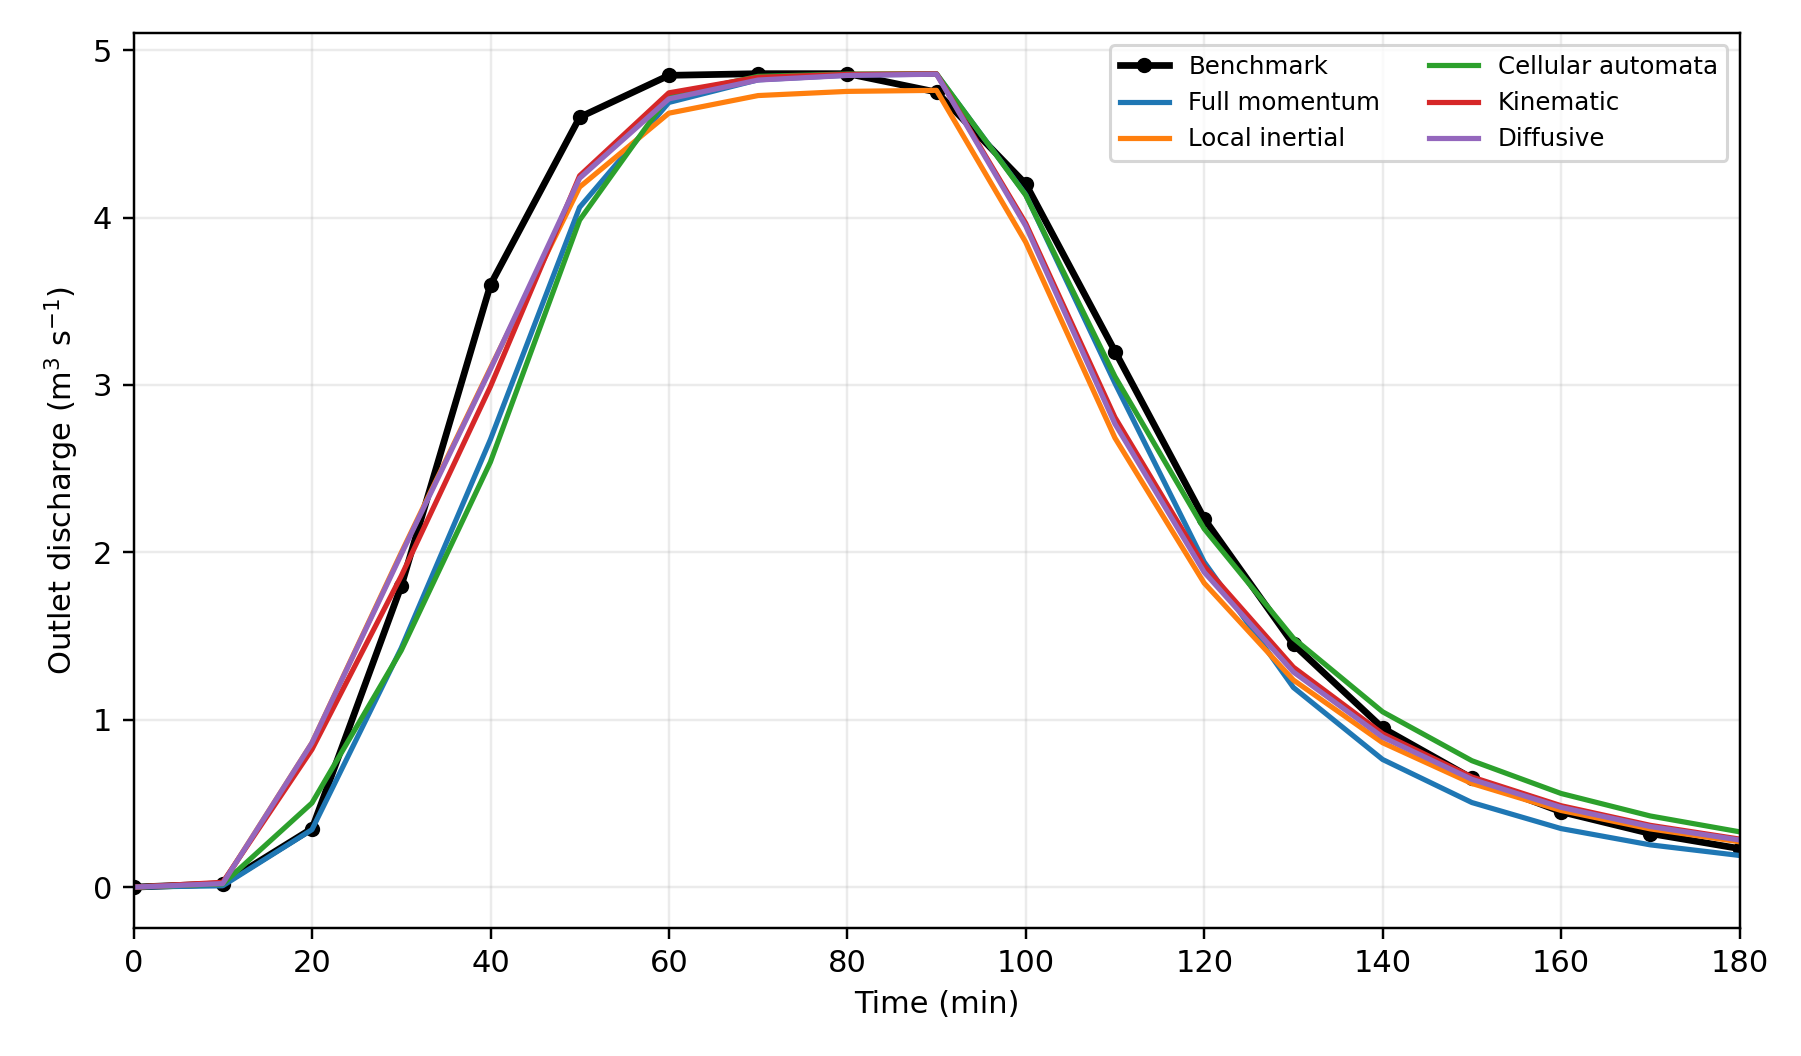
\includegraphics[width=\linewidth]{../static/validation/results/hydrodynamics/VAL_HYDRO_VTILT_ROUTING_HYDROGRAPH.png}
\caption{Canonical V-tilted benchmark hydrograph compared with the full-config \SI{20}{\meter} HydroPol2D full-momentum, local-inertial, cellular-automata, kinematic, and diffusive routing runs.}
\label{fig:val-hydro-li-vtilt-benchmark}
\end{figure}

\begin{figure}[htbp]
\centering
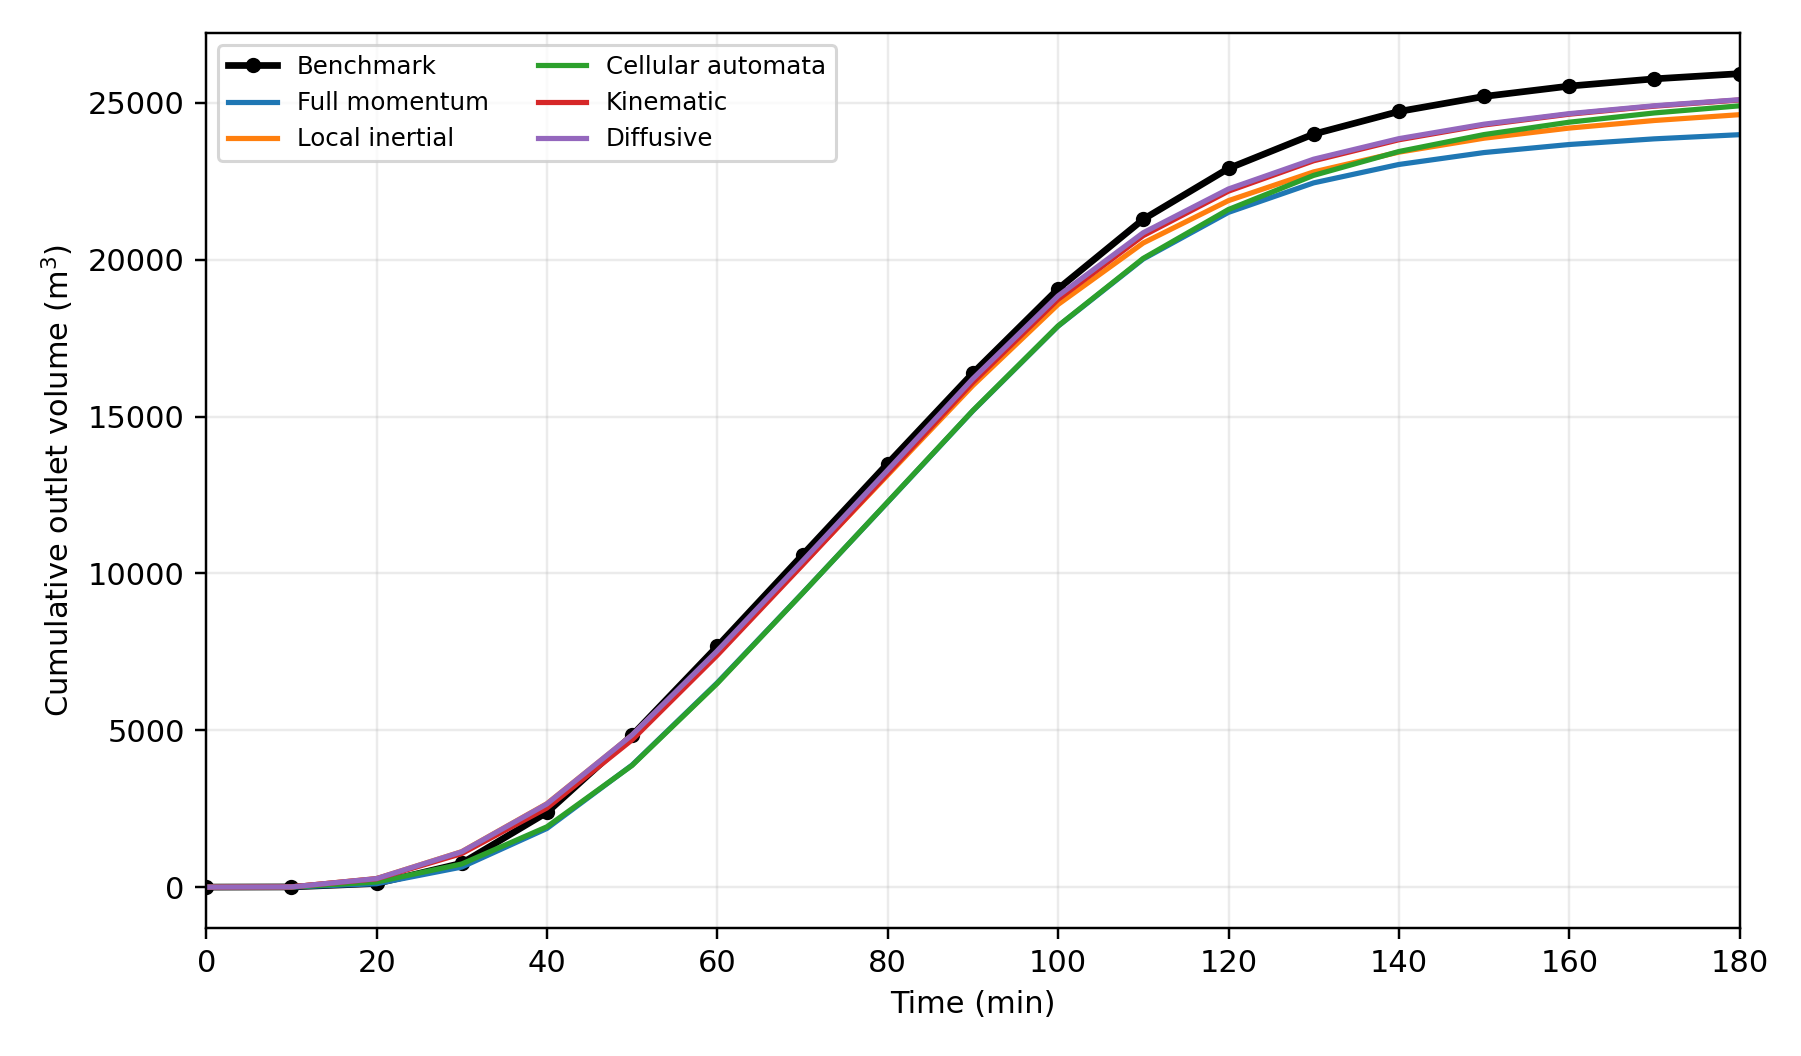
\includegraphics[width=0.82\linewidth]{../static/validation/results/hydrodynamics/VAL_HYDRO_VTILT_ROUTING_VOLUME.png}
\caption{Canonical V-tilted cumulative outlet-volume diagnostics for all full-config routing runs. The model ledger including final storage closes to \SI{-0.0181}{\percent} for every routing option.}
\label{fig:val-hydro-li-vtilt-volume}
\end{figure}

\begin{figure}[htbp]
\centering
\begin{minipage}{0.49\linewidth}
\centering
\includegraphics[width=\linewidth]{../../HydroPol2D/Validation/Hydrodynamics/LocalInertial_CA/Outputs/Validation/Figures/VAL_HYDRO_LI_PLANE_001.png}
\end{minipage}
\begin{minipage}{0.49\linewidth}
\centering
\includegraphics[width=\linewidth]{../../HydroPol2D/Validation/Hydrodynamics/LocalInertial_CA/Outputs/Validation/Figures/VAL_HYDRO_CA_PLANE_001.png}
\end{minipage}
\caption{Tilted-plane hydrograph diagnostics for local-inertial routing (left) and cellular-automata routing (right).}
\label{fig:val-hydro-li-ca-plane}
\end{figure}

\begin{figure}[htbp]
\centering
\begin{minipage}{0.49\linewidth}
\centering
\includegraphics[width=\linewidth]{../../HydroPol2D/Validation/Hydrodynamics/LocalInertial_CA/Outputs/Validation/Figures/VAL_HYDRO_LI_RITTER_001.png}
\end{minipage}
\begin{minipage}{0.49\linewidth}
\centering
\includegraphics[width=\linewidth]{../../HydroPol2D/Validation/Hydrodynamics/LocalInertial_CA/Outputs/Validation/Figures/VAL_HYDRO_CA_RITTER_001.png}
\end{minipage}
\caption{Ritter dam-break profile diagnostics for local-inertial routing (left) and cellular-automata routing (right). The local-inertial result is retained as a diagnostic failed benchmark.}
\label{fig:val-hydro-li-ca-ritter}
\end{figure}

\section{Routing Alternatives}
\label{sec:routing}
The kinematic and diffusive routing audit found two implementation-level problems. First, the kinematic solver declared the wrong primary function name, so MATLAB could not reliably dispatch it. Second, the old kinematic/diffusive bodies used copied slope logic with inconsistent row/column directions and a Manning flux expression that did not cleanly represent either bed-slope kinematic routing or water-surface-slope diffusive routing. These functions were replaced by a shared conservative D4 face-flux core. Kinematic routing now uses bed slope and upstream cell depth; diffusive routing uses water-surface slope with hydraulic reconstruction at cell faces. Both are updated by conservative finite-volume storage accounting, a draining limiter, outlet-volume bookkeeping, and internal substepping for steep fronts.

The corrected solvers were applied to the same validation sequence using \filepath{Validation/Hydrodynamics/Diffusive_Kinematic/run_diffusive_kinematic_hydrodynamics_validation.m}. The tilted-plane case is the primary analytical validation for the kinematic wave. The diffusive wave is compared with the same plane solution as an approximation benchmark and is also checked by conservation/symmetry on the v-tilted catchment. Ritter dam-break profiles are retained only as diagnostics because neither reduced equation solves the full dynamic-wave problem.

\begin{table}[htbp]
\centering
\caption{Corrected kinematic and diffusive routing metrics.}
\label{tab:routing-kinematic-diffusive-results}
\small
\setlength{\tabcolsep}{3pt}
\begin{tabular}{@{}L{0.14\textwidth}L{0.13\textwidth}R{0.11\textwidth}R{0.11\textwidth}R{0.08\textwidth}R{0.16\textwidth}L{0.14\textwidth}@{}}
\toprule
\rowcolor{HydroPale}
\thcell{Method} & \thcell{Case} & \thcell{RMSE} & \thcell{Relative\\$L_2$} & \thcell{NSE} & \thcell{Mass error\\ (\%)} & \thcell{Status} \\
\midrule
Kinematic & Plane & 0.0156 & 0.0184 & 0.9986 & $7.66\times10^{-12}$ & pass \\
Kinematic & V-tilted & 0.0000 & -- & -- & $4.18\times10^{-12}$ & pass \\
Kinematic & Ritter & 0.2408 & 0.5069 & 0.9245 & 0.0000 & diagnostic pass \\
Kinematic & Stage BC & 0.0000 & -- & -- & $1.32\times10^{-13}$ & pass \\
Diffusive & Plane & 0.0172 & 0.0203 & 0.9984 & $7.75\times10^{-12}$ & pass \\
Diffusive & V-tilted & 0.0000 & -- & -- & $3.73\times10^{-12}$ & pass \\
Diffusive & Ritter & 0.5670 & 1.1151 & -0.0803 & $1.53\times10^{-12}$ & diagnostic fail \\
Diffusive & Stage BC & 0.0000 & -- & -- & $1.58\times10^{-13}$ & pass \\
\bottomrule
\end{tabular}
\end{table}

The kinematic tilted-plane hydrograph reproduced the analytical kinematic-wave limit with NSE 0.9986 and relative $L_2$ error 0.0184. The diffusive plane run was similarly close for this mild rainfall-runoff case, with NSE 0.9984. Both solvers conserved mass to machine precision and preserved exact bilateral symmetry on the v-tilted catchment. The diffusive Ritter diagnostic failed, as expected for a reduced diffusive-wave approximation under a sharp dry-bed dam-break discontinuity; it is not used as validation evidence for diffusive routing.

\begin{figure}[htbp]
\centering
\begin{minipage}{0.49\linewidth}
\centering
\includegraphics[width=\linewidth]{../../HydroPol2D/Validation/Hydrodynamics/Diffusive_Kinematic/Outputs/Validation/Figures/VAL_HYDRO_KIN_PLANE_001.png}
\end{minipage}
\begin{minipage}{0.49\linewidth}
\centering
\includegraphics[width=\linewidth]{../../HydroPol2D/Validation/Hydrodynamics/Diffusive_Kinematic/Outputs/Validation/Figures/VAL_HYDRO_DIFF_PLANE_001.png}
\end{minipage}
\caption{Tilted-plane hydrograph validation for corrected kinematic routing (left) and corrected diffusive routing (right).}
\label{fig:val-route-kin-diff-plane}
\end{figure}

\section{Neal (2012) Channel-Subgrid Hydraulics}
\label{sec:subgrid}
HydroPol2D represents channels narrower than a raster cell with the rectangular channel formulation of \cite{Neal2012}. The channel is embedded below the coarse floodplain elevation. Channel and floodplain discharges are computed separately on each orthogonal face, then combined in the local-inertial continuity update. The supported configuration uses \texttt{flag\_inertial=1}, \texttt{flag\_subgrid=1}, and \texttt{flag\_overbanks=1}.

\subsection{Channel and Floodplain Formulation}
Let $\Delta x$ be the coarse-cell width, $z_f$ the floodplain elevation, $H$ the channel bank height, and $w$ the channel width, where $0<w<\Delta x$. The channel-bed elevation is
\begin{equation}
z_c=z_f-H.
\end{equation}
The representative depth $h$ is measured above $z_c$. For adjacent cells $i$ and $j$, the channel water surface $y_c=z_c+h$, face slope, and face depth are
\begin{equation}
S_c=\frac{y_{c,j}-y_{c,i}}{\Delta x},
\qquad
h_{c,f}=\max\left[\max(y_{c,i},y_{c,j})-\max(z_{c,i},z_{c,j}),0\right].
\end{equation}
The shared channel width, flow area, and hydraulic radius are
\begin{equation}
w_{c,f}=\min(w_i,w_j),
\qquad A_c=w_{c,f}h_{c,f},
\qquad R_c=\frac{A_c}{w_{c,f}+2h_{c,f}}.
\end{equation}
The channel discharge is updated as
\begin{equation}
Q_c^{t+\Delta t}=\frac{Q_c^t-gA_c\Delta t S_c}
{1+g\Delta t n_c^2|Q_c^t|/(R_c^{4/3}A_c)},
\end{equation}
where $n_c$ is the channel Manning coefficient.

Floodplain depth is $h_f=\max(h+z_c-z_f,0)$. The corresponding face slope $S_f$ and face depth $h_{f,f}$ are computed from the floodplain water surface $y_f=z_f+h_f$. Floodplain unit discharge is
\begin{equation}
q_f^{t+\Delta t}=\frac{q_f^t-gh_{f,f}\Delta t S_f}
{1+g\Delta t n_f^2|q_f^t|/h_{f,f}^{7/3}},
\end{equation}
where $n_f$ is the floodplain Manning coefficient. Total floodplain and face discharges are
\begin{equation}
Q_f=q_f(\Delta x-w_{c,f}),
\qquad Q=Q_c+Q_f.
\end{equation}

Cell continuity is evaluated in volume space. The storage relation is
\begin{equation}
V(h)=
\begin{cases}
\Delta x\,w\,h, & h\le H,\\
\Delta x\,w\,H+\Delta x^2(h-H), & h>H.
\end{cases}
\end{equation}
Routing fluxes and hydrologic sources or sinks update $V$ first. The same piecewise relation is then inverted to recover $h$. Thus, the active surface area changes conservatively from $\Delta xw$ in-bank to $\Delta x^2$ overbank.

\subsection{Numerical-reference Protocol}
Each retained case compares three local-inertial simulations: a fine grid that resolves channel and floodplain topography, an ordinary coarse grid without an embedded channel, and a coarse grid with the Neal (2012) formulation. The fine grid is a numerical reference, not an analytical solution. The comparison tests whether the embedded channel preserves hydraulic behavior that is lost when the grid is coarsened.

\subsection{Simple In-bank Channel}
Cases \texttt{VAL-SUBGRID-NEAL-SIMPLE-001} and \texttt{VAL-SUBGRID-NEAL-SIMPLE-002} use a \SI{10}{\meter}-wide, \SI{1}{\meter}-deep channel with bed slope 0.001 and Manning $n=0.035$. The explicit grid has \SI{10}{\meter} cells; the ordinary and Neal (2012) grids have \SI{30}{\meter} cells. A constant \SI{5}{\cubic\meter\per\second} inflow remains within bank.

For the 30-cell reach, the Neal (2012) hydrograph RMSE is \SI{0.098}{\cubic\meter\per\second}, compared with \SI{0.677}{\cubic\meter\per\second} for the ordinary coarse grid. NSE increases from 0.561 to 0.991, and stage RMSE decreases from \SI{0.689}{\meter} to \SI{0.053}{\meter}. The embedded channel corrects the excessive flow width and storage represented by the ordinary coarse cells.

\begin{figure}[htbp]
\centering
\begin{minipage}{0.49\linewidth}
\centering
\includegraphics[width=\linewidth]{../../HydroPol2D/Validation/Subgrid/Neal2012_SimpleStraightChannel/Figures/VAL-SUBGRID-NEAL-SIMPLE-002_HydrographStage.png}
\end{minipage}
\begin{minipage}{0.49\linewidth}
\centering
\includegraphics[width=\linewidth]{../../HydroPol2D/Validation/Subgrid/Neal2012_SimpleStraightChannel/Figures/VAL-SUBGRID-NEAL-SIMPLE-002_Profile.png}
\end{minipage}
\caption{Simple in-bank channel benchmark. The Neal (2012) coarse grid reproduces the fine-grid hydrograph, internal stage, and longitudinal profile more closely than the ordinary coarse grid.}
\label{fig:val-subgrid-neal-simple}
\end{figure}

\subsection{Composite Channel Under Constant and Transient Inflow}
The composite case uses a \SI{990}{\meter} reach with a \SI{10}{\meter}-wide, \SI{1}{\meter}-deep channel, \SI{90}{\meter} lateral benches, slope 0.005, and Manning $n=0.035$. The explicit reference uses \SI{10}{\meter} cells, and both coarse simulations use \SI{30}{\meter} cells. Constant \SI{100}{\cubic\meter\per\second} inflow and a Nash hydrograph peaking at \SI{100}{\cubic\meter\per\second} at \SI{30}{\minute} were tested.

\begin{table}[htbp]
\centering
\caption{Composite-channel metrics relative to the \SI{10}{\meter} explicit numerical reference.}
\label{tab:val-subgrid-neal-composite}
\small
\begin{tabular}{llrrrr}
\toprule
Forcing & Coarse model & Outlet RMSE & Outlet NSE & Internal RMSE & Storage RMSE \\
& & (\si{\cubic\meter\per\second}) & & (\si{\cubic\meter\per\second}) & (\si{\cubic\meter}) \\
\midrule
Constant & Ordinary & 6.178 & 0.954 & 4.819 & 2439 \\
Constant & Neal (2012) & 4.189 & 0.979 & 3.346 & 734 \\
Nash & Ordinary & 7.263 & 0.949 & 5.770 & 3363 \\
Nash & Neal (2012) & 4.044 & 0.984 & 2.987 & 781 \\
\bottomrule
\end{tabular}
\end{table}

\begin{figure}[htbp]
\centering
\includegraphics[width=0.9\linewidth]{../../HydroPol2D/Validation/Subgrid/Neal2012_CompositeChannel_100cms/Figures/NashTransient/CompositeChannel_Hydrographs.png}
\caption{Transient composite-channel comparison. The \SI{30}{\meter} Neal (2012) simulation follows the \SI{10}{\meter} explicit outlet and internal hydrographs more closely than the ordinary \SI{30}{\meter} simulation.}
\label{fig:val-subgrid-neal-composite}
\end{figure}

\subsection{Staged Overbank Flow}
Case \texttt{VAL-SUBGRID-NEAL-STAGED-OVERBANK-001} evaluates channel-to-floodplain activation. The \SI{1}{\kilo\meter} reach is \SI{300}{\meter} wide with slope 0.005. Its cross section has a \SI{50}{\meter} channel, two \SI{25}{\meter} benches at \SI{0.5}{\meter} above the channel bed, and an external floodplain at \SI{1.0}{\meter}. Channel Manning $n$ is 0.035 and floodplain Manning $n$ is 0.10. The explicit reference uses \SI{5}{\meter} cells; the ordinary and Neal (2012) grids use \SI{100}{\meter} cells. The Nash inflow peaks at \SI{200}{\cubic\meter\per\second} at \SI{45}{\minute}. Analytical uniform-flow calculations give activation discharges of \SI{31.4}{\cubic\meter\per\second} for the benches and \SI{110.8}{\cubic\meter\per\second} for the external floodplain.

\begin{figure}[htbp]
\centering
\includegraphics[width=0.9\linewidth]{../../HydroPol2D/Validation/Subgrid/Neal2012_StagedOverbank_100m/Figures/Geometry_and_AnalyticalRating.png}
\caption{Staged compound-channel geometry and analytical uniform-flow rating curve. The inflow activates both the internal benches and the external floodplain.}
\label{fig:val-subgrid-neal-staged-geometry}
\end{figure}

\begin{table}[htbp]
\centering
\caption{Staged-overbank metrics relative to the \SI{5}{\meter} explicit numerical reference.}
\label{tab:val-subgrid-neal-staged}
\begin{tabular}{lrr}
\toprule
Metric & Ordinary \SI{100}{\meter} & Neal (2012) \SI{100}{\meter} \\
\midrule
Outlet RMSE (\si{\cubic\meter\per\second}) & 15.476 & 2.723 \\
Outlet NSE & 0.945 & 0.998 \\
Internal RMSE (\si{\cubic\meter\per\second}) & 12.053 & 3.043 \\
Bench-depth RMSE (m) & 0.180 & 0.018 \\
Maximum-depth RMSE (m) & 0.280 & 0.040 \\
Wet-area CSI at \SI{0.01}{\meter} & 0.334 & 0.998 \\
\bottomrule
\end{tabular}
\end{table}

The Neal (2012) simulation activates the benches at \SI{21}{\minute}, equal to the explicit reference, and the external floodplain at \SI{35}{\minute}, compared with \SI{34}{\minute} in the reference. Its outlet hydrograph, depth series, and maximum inundation extent are substantially closer to the reference than those from the ordinary \SI{100}{\meter} grid. All retained Neal (2012) cases have mass residuals below $6\times10^{-13}$\%.

\begin{figure}[htbp]
\centering
\includegraphics[width=0.9\linewidth]{../../HydroPol2D/Validation/Subgrid/Neal2012_StagedOverbank_100m/Figures/Hydrograph_Comparison.png}
\caption{Staged-overbank outlet and internal hydrographs. The Neal (2012) result follows the fine-grid reference through activation and peak flow.}
\label{fig:val-subgrid-neal-staged-hydrograph}
\end{figure}

\begin{figure}[htbp]
\centering
\includegraphics[width=\linewidth]{../../HydroPol2D/Validation/Subgrid/Neal2012_StagedOverbank_100m/Figures/MaximumDepth_Maps.png}
\caption{Maximum-depth maps for the staged-overbank case. The ordinary coarse grid underestimates floodplain wetting, whereas the Neal (2012) result approaches the fine-grid maximum extent.}
\label{fig:val-subgrid-neal-staged-depth}
\end{figure}

The staged case also defines the present limitation. The Neal (2012) benches become dry at \SI{126}{\minute}, compared with \SI{196}{\minute} in the explicit reference. The external floodplain becomes dry at \SI{152}{\minute}, compared with \SI{237}{\minute}. One representative water level is stored in each coarse channel cell, so residual water on benches and floodplains cannot drain independently from the embedded channel. The controlled tests therefore support in-bank routing, floodplain activation, peak hydraulics, and maximum extent within the tested geometries. Applications controlled by late floodplain drainage require separate observational or fine-grid evaluation.

\section{Reservoir and Control Structures}
\label{sec:reservoirs}
The reservoir validation isolates the control-structure rating-curve logic before it is coupled to a full catchment. The benchmark uses a constant-area reservoir with storage $S=A h$ and a single outlet rating curve
\begin{equation}
Q = k\max(h-h_0,0)^b ,
\end{equation}
where $h$ is reservoir stage, $h_0$ is the sill stage, $k$ is the rating coefficient, and $b$ is the rating exponent. With no external inflow, the analytical reference is the exact depletion solution of
\begin{equation}
A\frac{dh}{dt}=-k(h-h_0)^b .
\end{equation}
For $b \neq 1$, this gives
\begin{equation}
h(t)=h_0+\left[(h(0)-h_0)^{1-b}+(b-1)\frac{k}{A}t\right]^{1/(1-b)} .
\end{equation}
The implemented test in \filepath{Validation/Reservoir/RatingCurve_StorageDepletion/run_reservoir_rating_curve_validation.m} uses $A=\SI{20000}{\square\meter}$, $h(0)=\SI{2.50}{\meter}$, $h_0=\SI{0.35}{\meter}$, $k=2.2$, and $b=1.5$. The explicit HydroPol2D rating-step update is compared against the exact stage, storage, and discharge series.

\begin{table}[htbp]
\centering
\caption{Reservoir rating-curve validation metrics.}
\label{tab:val-reservoir-metrics}
\small
\setlength{\tabcolsep}{2.5pt}
\begin{tabular}{@{}L{0.14\textwidth}R{0.18\textwidth}R{0.18\textwidth}R{0.11\textwidth}R{0.16\textwidth}R{0.14\textwidth}@{}}
\toprule
\rowcolor{HydroPale}
\thcell{Case} & \thcell{Storage RMSE\\ (\si{\cubic\meter})} & \thcell{Outflow RMSE\\ (\si{\cubic\meter\per\second})} & \thcell{Relative\\$L_2$} & \thcell{Recovered $k$ error\\ (\%)} & \thcell{Mass residual\\ (\%)} \\
\midrule
VAL-RES-001 & 0.2730 & $4.96\times10^{-5}$ & $7.80\times10^{-6}$ & 0.0000 & $4.37\times10^{-13}$ \\
\bottomrule
\end{tabular}
\end{table}

The case passed all thresholds. The small storage difference is the expected explicit-integration truncation error relative to the continuous exact ODE, while the mass ledger itself closes to numerical precision because released volume plus remaining storage equals the initial storage.

\begin{figure}[htbp]
\centering
\includegraphics[width=\linewidth]{../../HydroPol2D/Validation/Reservoir/RatingCurve_StorageDepletion/Outputs/Validation/Figures/VAL_RES_001_RATING_CURVE.png}
\caption{Reservoir rating-curve validation. The upper panel compares modeled and exact stage depletion, the middle panel compares rating-curve discharge, and the lower panel reports storage error and mass residual.}
\label{fig:val-reservoir-ode}
\end{figure}

\section{Inflow Hydrograph Boundary Conditions}
\label{sec:boundary-inflow}
The inflow hydrograph boundary test imposes a known triangular hydrograph on the upstream boundary of a rectangular full-momentum domain. This is a boundary-condition validation rather than a dam-break validation: breach-style hydrographs, when needed, should be supplied through this same inflow-hydrograph mechanism. The truth source is the exact integral of the prescribed hydrograph. The routed downstream hydrograph is diagnostic because no analytical Saint-Venant solution is expected for the finite rough rectangular domain.

The implemented case in \filepath{Validation/BoundaryConditions/InflowHydrograph_RectangularDomain/run_inflow_hydrograph_validation.m} imposes a hydrograph that starts at \SI{5}{\minute}, peaks at \SI{25}{\minute} with \SI{8}{\cubic\meter\per\second}, and returns to zero at \SI{45}{\minute}. The exact inflow volume is \SI{9600}{\cubic\meter}. The full-momentum domain routes the wave to a downstream outlet while the diagnostic ledger checks
\begin{equation}
V_{\mathrm{in}} = V_{\mathrm{out}} + S_{\mathrm{domain}} + \epsilon .
\end{equation}

\begin{table}[htbp]
\centering
\caption{Inflow-hydrograph boundary validation metrics.}
\label{tab:val-inflow-bc-metrics}
\small
\setlength{\tabcolsep}{2pt}
\begin{tabular}{@{}L{0.16\textwidth}R{0.14\textwidth}R{0.14\textwidth}R{0.15\textwidth}R{0.12\textwidth}R{0.16\textwidth}@{}}
\toprule
\rowcolor{HydroPale}
\thcell{Case} & \thcell{Imposed\\volume error\\(\%)} & \thcell{Mass residual\\ (\%)} & \thcell{Outlet peak\\ (\si{\cubic\meter\per\second})} & \thcell{Peak lag\\ (\si{\minute})} & \thcell{Peak magnitude\\error (\%)} \\
\midrule
VAL-BC-INFLOW-001 & $3.41\times10^{-13}$ & $6.44\times10^{-13}$ & 7.3771 & 5.0 & 7.7862 \\
\bottomrule
\end{tabular}
\end{table}

The case passed the imposed-volume and water-balance criteria. At the end of the \SI{3}{\hour} run, \SI{9579.14}{\cubic\meter} had exited the outlet and \SI{20.86}{\cubic\meter} remained stored in the domain, closing the ledger against the \SI{9600}{\cubic\meter} imposed inflow volume.

\begin{figure}[htbp]
\centering
\includegraphics[width=\linewidth]{../../HydroPol2D/Validation/BoundaryConditions/InflowHydrograph_RectangularDomain/Outputs/Validation/Figures/VAL_BC_INFLOW_001_HYDROGRAPH.png}
\caption{Inflow-hydrograph boundary validation under full-momentum routing. The upper panel shows the prescribed inflow and routed downstream hydrograph, the middle panel compares cumulative volumes, and the lower panel reports stored volume and mass residual.}
\label{fig:val-inflow-bc}
\end{figure}

\section{Stage Hydrograph Boundary Conditions}
\label{sec:boundary-stage}
The stage-hydrograph cases prescribe a sinusoidal upstream boundary depth in a rectangular domain. At every model step the upstream stage cells are reset to the prescribed value, the selected routing solver propagates the perturbation, and the diagnostic ledger tracks the volume inserted or removed by the stage boundary, outlet volume, and remaining domain storage. The prescribed boundary-stage enforcement error was zero to numerical precision for full momentum, local inertial, CA, kinematic, and diffusive routing. The downstream response amplitudes were \SI{0.0718}{\meter}, \SI{0.0723}{\meter}, \SI{0.0170}{\meter}, \SI{0.1514}{\meter}, and \SI{0.0964}{\meter}, respectively, with all water-balance errors far below \SI{0.1}{\percent}.

\begin{figure}[htbp]
\centering
\includegraphics[width=\linewidth]{../../HydroPol2D/Validation/Hydrodynamics/FullMomentum/Outputs/Validation/Figures/VAL_BC_STAGE_FM_001.png}
\caption{Prescribed stage-hydrograph boundary validation under full-momentum routing. The upper panel shows the imposed upstream stage and downstream response; the lower panel shows the mass-balance residual.}
\label{fig:val-bc-stage-fm}
\end{figure}

\begin{figure}[htbp]
\centering
\begin{minipage}{0.49\linewidth}
\centering
\includegraphics[width=\linewidth]{../../HydroPol2D/Validation/Hydrodynamics/LocalInertial_CA/Outputs/Validation/Figures/VAL_BC_STAGE_LI_001.png}
\end{minipage}
\begin{minipage}{0.49\linewidth}
\centering
\includegraphics[width=\linewidth]{../../HydroPol2D/Validation/Hydrodynamics/LocalInertial_CA/Outputs/Validation/Figures/VAL_BC_STAGE_CA_001.png}
\end{minipage}
\caption{Prescribed stage-hydrograph boundary validation under local-inertial routing (left) and cellular-automata routing (right).}
\label{fig:val-bc-stage-li-ca}
\end{figure}

\begin{figure}[htbp]
\centering
\begin{minipage}{0.49\linewidth}
\centering
\includegraphics[width=\linewidth]{../../HydroPol2D/Validation/Hydrodynamics/Diffusive_Kinematic/Outputs/Validation/Figures/VAL_BC_STAGE_KIN_001.png}
\end{minipage}
\begin{minipage}{0.49\linewidth}
\centering
\includegraphics[width=\linewidth]{../../HydroPol2D/Validation/Hydrodynamics/Diffusive_Kinematic/Outputs/Validation/Figures/VAL_BC_STAGE_DIFF_001.png}
\end{minipage}
\caption{Prescribed stage-hydrograph boundary validation under corrected kinematic routing (left) and corrected diffusive routing (right).}
\label{fig:val-bc-stage-kin-diff}
\end{figure}

\section{Spatial Rainfall and Satellite Maps}
\label{sec:spatial-rainfall}
The spatial-rainfall case validates raster ingestion, temporal accumulation, unit conversion, and cellwise volume accounting before these rainfall maps are coupled to routing, infiltration, or ET. Stanford remains an applied invariant-rainfall example; it is not used as the spatial-rainfall truth case.

The implemented benchmark in \filepath{Validation/SpatialRainfall/TinyRaster_TotalRainfall/run_spatial_rainfall_raster_validation.m} writes three tiny GeoTIFF rainfall-intensity rasters on a \num{4} by \num{5} grid with \SI{20}{\meter} cells. The rasters are prescribed in \si{\milli\meter\per\hour} and assigned durations of \SI{10}{\minute}, \SI{20}{\minute}, and \SI{15}{\minute}. The reference accumulated depth in each cell is
\begin{equation}
P_{i,j} = \sum_k \frac{I_{i,j,k}}{1000}\frac{\Delta t_k}{60},
\end{equation}
and the domain volume is
\begin{equation}
V_P = \sum_{i,j} P_{i,j}\Delta x^2 .
\end{equation}
This case intentionally includes spatial gradients and zero-rainfall cells to expose row/column flips, domain averaging, missing no-data handling, and timestep-unit mistakes.

\begin{table}[htbp]
\centering
\caption{Spatial rainfall raster validation metrics.}
\label{tab:val-raster-rain-metrics}
\small
\setlength{\tabcolsep}{2.5pt}
\begin{tabular}{@{}L{0.16\textwidth}R{0.14\textwidth}R{0.14\textwidth}R{0.17\textwidth}R{0.14\textwidth}R{0.14\textwidth}@{}}
\toprule
\rowcolor{HydroPale}
\thcell{Case} & \thcell{Cellwise RMSE\\ (\si{\meter})} & \thcell{Maximum cell\\error (\si{\meter})} & \thcell{Total volume\\ (\si{\cubic\meter})} & \thcell{Volume error\\ (\%)} & \thcell{Maximum step\\error (\%)} \\
\midrule
VAL-RAIN-MAP-001 & 0 & 0 & 75.3333 & 0 & 0 \\
\bottomrule
\end{tabular}
\end{table}

The case passed exactly: the raster-read accumulated depths matched the prescribed cellwise reference, each timestep volume matched the analytical integral, and the total rainfall volume residual was zero.

\begin{figure}[htbp]
\centering
\includegraphics[width=\linewidth]{../../HydroPol2D/Validation/SpatialRainfall/TinyRaster_TotalRainfall/Outputs/Validation/Figures/VAL_RAIN_MAP_001_TOTALS.png}
\caption{Spatial rainfall raster validation. The panels compare prescribed accumulated rainfall, raster-read accumulated rainfall, cellwise error, and stepwise rainfall volumes.}
\label{fig:val-raster-rain}
\end{figure}

\section{Water Quality}
\label{sec:water-quality}
The water-quality case validates HydroPol2D's current mass-based buildup/washoff pathway before any field pollutograph calibration is attempted. The case uses physically plausible total suspended solids (TSS) parameter scales from the EPA SWMM buildup/washoff framework \cite{Rossman2015SWMMUser,RossmanHuber2016SWMMWQ}, but the truth source is analytical mass balance rather than a SWMM numerical run.

The validation driver is \filepath{Validation/WaterQuality/BuildUpWashOff_MassBalance/run_water_quality_washoff_validation.m}. It calls HydroPol2D's \texttt{build\_up\_wash\_off.m} directly in \texttt{flag\_wq\_model = 0} mass-based washoff mode. Three deterministic checks are included: dry-weather buildup initialization, single-cell exponential washoff, and conservative two-cell transfer/export. The TSS-like setup uses a \SI{400}{\square\meter} cell, \SI{30}{\milli\meter\per\hour} runoff, a maximum buildup scale of \SI{56.04}{\kilogram\per\hectare} (about \SI{50}{lb/acre}), \SI{5}{day} antecedent dry weather, and a washoff coefficient selected to give an initial concentration of about \SI{120}{\milli\gram\per\liter}, within a plausible urban first-flush range.

Dry-weather buildup follows the SWMM-style exponential form
\begin{equation}
B_0 = C_1 \left(1-\exp(-C_2 ADD)\right)\frac{A}{10000},
\end{equation}
where $C_1$ is the maximum buildup in \si{\kilogram\per\hectare}, $C_2$ is the buildup rate in \si{\per\day}, $ADD$ is antecedent dry days, and $A$ is cell area in \si{\square\meter}. For the HydroPol2D mass-based washoff mode, the removed pollutant load is
\begin{equation}
W = C_3 Q^{C_4} B,
\end{equation}
where $B$ is remaining pollutant mass, $Q$ is runoff discharge, and $C_4=1$ in this validation. Under constant runoff, the analytical single-cell solution is
\begin{equation}
B(t) = B_0 \exp(-\lambda t), \qquad \lambda = C_3 Q^{C_4},
\end{equation}
with $t$ in hours for this driver. The two-cell transfer case uses identical first-order washoff in both cells. With equal initial masses $B_0$ in the upstream and downstream cells, the analytical cell masses are
\begin{equation}
B_1(t)=B_0\exp(-\lambda t), \qquad
B_2(t)=\exp(-\lambda t)\left(B_0+\lambda B_0 t\right),
\end{equation}
and exported mass is obtained by conservation.

The validation exposed an implementation artifact: the mass-based washoff routines rounded remaining pollutant mass to six decimal places at every substep. That quantization accumulated into an artificial mass error in high-resolution analytical tests. The routines now preserve full precision and only clean near-zero roundoff values. Table~\ref{tab:val-wq-metrics} reports the passing current-code metrics after that correction.

\begin{table}[htbp]
\centering
\caption{Water-quality buildup/washoff validation metrics.}
\label{tab:val-wq-metrics}
\begin{tabular}{lrrrr}
\toprule
Case & Mass RMSE (kg) & Export error (\%) & Mass residual (kg) & Negative mass count \\
\midrule
Dry-weather buildup & 0 & 0 & 0 & 0 \\
Single-cell washoff & $4.998\times10^{-7}$ & $2.483\times10^{-4}$ & 0 & 0 \\
Two-cell transfer & $6.272\times10^{-8}$ & $3.722\times10^{-5}$ & 0 & 0 \\
\bottomrule
\end{tabular}
\end{table}

All three cases passed the validation acceptance thresholds: mass RMSE below \SI{1e-6}{\kilogram}, exported-load error below \SI{0.01}{\percent}, zero mass residual, no negative mass, and no unexplained \texttt{NaN} values. Figures~\ref{fig:val-wq-single} and~\ref{fig:val-wq-two-cell} show the analytical comparisons and conservation ledgers for the single-cell and two-cell cases.

\begin{figure}[htbp]
\centering
\includegraphics[width=\linewidth]{../../HydroPol2D/Validation/WaterQuality/BuildUpWashOff_MassBalance/Outputs/Validation/Figures/VAL_WQ_001_SINGLE_CELL.png}
\caption{Single-cell water-quality validation. HydroPol2D's mass-based washoff is compared with the exact exponential remaining-mass, load, concentration, and cumulative-export solution under constant runoff.}
\label{fig:val-wq-single}
\end{figure}

\begin{figure}[htbp]
\centering
\includegraphics[width=\linewidth]{../../HydroPol2D/Validation/WaterQuality/BuildUpWashOff_MassBalance/Outputs/Validation/Figures/VAL_WQ_001_TWO_CELL.png}
\caption{Two-cell water-quality validation. Upstream washoff enters the downstream cell, downstream washoff exits the domain, and remaining plus exported pollutant mass closes exactly.}
\label{fig:val-wq-two-cell}
\end{figure}

\section{Human Risk and Instability}
\label{sec:human-risk}
The human-risk case validates the implemented algebra and classification logic, not field-scale public-safety prediction. The driver \filepath{Validation/HumanRisk/DepthVelocity_Classification/run_human_risk_instability_validation.m} tests two active HydroPol2D pathways. The first is the simple instability index used when \texttt{flag\_human\_instability = 1}. The second is the detailed force-balance classifier used when \texttt{flag\_human\_instability = 3}, which returns stable, sliding, toppling, or drowning classes.

For the simple instability index, the independent reference computes person weight, buoyancy, available friction, and hydrodynamic drag:
\begin{equation}
F_p = mg, \qquad
F_b = w_1 w_2 h \rho_w g,
\end{equation}
\begin{equation}
F_f = \mu \max(F_p-F_b,0), \qquad
F_d = \frac{1}{2} C_d \rho_w w_1 h v^2.
\end{equation}
The reported risk index is
\begin{equation}
R = \min\left(\frac{F_d}{F_f},1\right),
\end{equation}
with a deterministic edge convention: dry cells have $R=0$, while wet cells with no available friction have $R=1$. This convention avoids the physically ambiguous \texttt{0/0} case that previously produced \texttt{NaN} for still water when buoyancy eliminated friction.

For the detailed classifier, an independent implementation of the same slide, topple, and drowning force-balance equations was evaluated over a depth/velocity grid. The grid includes exact geometry-split and drowning-threshold cases. The geometry split is deterministic at equality by assigning the exact split depth to the lower-depth branch. The drowning threshold uses the implemented open condition $h > 13y/16$, so the exact threshold is not yet classified as drowning, while any value above it is.

\begin{table}[htbp]
\centering
\caption{Human-risk and instability validation metrics.}
\label{tab:val-hr-metrics}
\begin{tabular}{lrrrrr}
\toprule
Case & RMSE & Max error & Accuracy (\%) & Boundary errors & NaN count \\
\midrule
Simple instability index & 0 & 0 & 100 & 0 & 0 \\
Slide/topple/drowning classifier & 0 & 0 & 100 & 0 & 0 \\
\bottomrule
\end{tabular}
\end{table}

The detailed classifier grid exercised all implemented output classes: 21 stable cells, 19 sliding cells, 2 toppling cells, and 12 drowning cells. All model classes matched the independent reference. Figures~\ref{fig:val-hr-simple} and~\ref{fig:val-hr-force} show the model outputs and zero-error maps.

\begin{figure}[htbp]
\centering
\includegraphics[width=\linewidth]{../../HydroPol2D/Validation/HumanRisk/DepthVelocity_Classification/Outputs/Validation/Figures/VAL_HR_001_SIMPLE_INSTABILITY.png}
\caption{Simple human-instability validation. The left panel shows the HydroPol2D instability index over the deterministic depth/velocity grid; the right panel shows model-reference error.}
\label{fig:val-hr-simple}
\end{figure}

\begin{figure}[htbp]
\centering
\includegraphics[width=\linewidth]{../../HydroPol2D/Validation/HumanRisk/DepthVelocity_Classification/Outputs/Validation/Figures/VAL_HR_001_FORCE_BALANCE.png}
\caption{Detailed human-risk classifier validation. The left panel shows stable, sliding, toppling, and drowning classes; the right panel shows zero classification error against the independent force-balance reference.}
\label{fig:val-hr-force}
\end{figure}

\section{Discussion}
\label{sec:discussion}
The validation suite deliberately separates isolated formula checks from coupled-domain dynamics. This prevents a correct final hydrograph from masking compensating errors among rainfall input, interception, infiltration, ET, groundwater exchange, routing, and boundary handling. At this stage, report-ready claims are limited to modules that have current-code outputs, documented analytical or independent-reference targets, exact bookkeeping checks, and standardized diagnostics.

\section{Limitations}
\label{sec:limitations}
This validation report contains completed module results for canopy interception, snow, infiltration, evapotranspiration, groundwater and recharge, hydrodynamics, routing alternatives, Neal (2012) channel-subgrid hydraulics, reservoirs, boundary conditions, spatial rainfall, water quality, and human risk. Local-inertial routing did not pass the Ritter dam-break analytical threshold and should not be cited as validated for dam-break dynamics. Kinematic and diffusive routing passed their reduced-equation plane, conservation, stage-bookkeeping, and V-tilted tests, but their Ritter cases remain diagnostic. The Neal (2012) channel-subgrid results use fine-grid local-inertial simulations as numerical references. They support the tested in-bank, channel-to-floodplain activation, peak-flow, and maximum-inundation behavior. They do not establish field-scale accuracy. The staged case also shows that one water level per coarse cell can make benches and floodplains drain too quickly during late recession.

\section{Final Summary}
\label{sec:summary}
The validation suite proceeds from canopy interception through snow, infiltration, evapotranspiration, groundwater, hydrodynamics, reservoirs, boundary conditions, spatial rainfall, water quality, and risk classification. The completed cases pass their analytical, independent-reference, numerical-reference, or exact-bookkeeping criteria within the stated scope. The local-inertial and diffusive Ritter comparisons remain failed diagnostics, and the kinematic Ritter comparison remains diagnostic rather than a dynamic-wave validation claim. The Neal (2012) channel-subgrid formulation improves hydrograph, stage, storage, and inundation metrics relative to the ordinary coarse grid in all retained controlled cases. In the staged-overbank test, outlet NSE is 0.998, maximum-depth RMSE is \SI{0.040}{\meter}, and wet-area CSI is 0.998. The main remaining limitation is early late-stage drainage from coarse floodplain cells. Field calibration and observational validation remain outside validation.

\bibliographystyle{plain}
\bibliography{references}

\end{document}
